\documentclass[]{article}

\usepackage[english]{babel}
\usepackage[utf8x]{inputenc}
\usepackage{amsthm,amsmath,amssymb,amsfonts}
\usepackage{geometry}
\geometry{
	a4paper,
 total={150mm,257mm},
 left=30mm,
 top=20mm,
}
\usepackage{booktabs,threeparttable,threeparttablex}
\usepackage{multirow}
\usepackage[labelsep=endash, skip=5pt]{caption}
\usepackage{graphicx}
\usepackage{setspace}
\usepackage{natbib}
\usepackage{hyperref}
\Urlmuskip=0mu  plus 10mu
\usepackage{xurl}
\usepackage{lmodern,textcomp} % for euro symbol
\hypersetup{
    colorlinks=true,
    linkcolor=blue,
    filecolor=blue,      
    urlcolor=gray,
    citecolor=blue,
    pdftitle={Sharelatex Example},
    pdfpagemode=FullScreen,
    }
\usepackage{enumerate}
\usepackage[colorinlistoftodos]{todonotes}
\usepackage{subcaption}
\usepackage{float}
\usepackage[justification=centering]{caption}
\usepackage{tikz}
\usetikzlibrary{decorations.pathreplacing}

\usepackage{soul}


\newcommand{\sa}{s^0(\alpha,p^*)}
\newcommand{\sd}{p^*}
\newcommand{\B}{\mbox{Br}}
\newcommand{\sn}{s^{*}(\alpha)}
\newcommand{\ft}{F^{tacit}}
\newcommand{\fc}{F^{com}}
\newcommand{\E}{\mathbb E}

\newtheorem{lemma}{Lemma}
\newtheorem{proposition}{Proposition}
\newtheorem{corollary}{Corollary}
\newtheorem{assumption}{Assumption}
\newtheorem{example}{Example}
\newtheorem{definition}{Definition}

\newcommand{\p}{\mathbf p}

\title{Let's Collude\footnote{We benefited from comments of audiences at ECARES, CRESSE, EARIE, IIOC and BECCLE, with special thanks to Estelle Cantillon, Georg Kirchteiger, Kai-Uwe K\"uhn and Joseph Harrington. This research has benefited from the financial support of the European Research Council under the European Union's Seventh Framework Programme (FP7/2007-2013 / ERC grant agreement 339950.) Hamid Aghadadashli was a postdoc at ECARES during the completion of this project.}}
\author{{\Large Hamid Aghadadashli\thanks{Universit\'e libre de Bruxelles (ECARES). Present address: NERA Economic Consulting, Germany; e-mail: \href{mailto:aghadadashli@me.com}{aghadadashli@me.com}
.}}
\and {\Large Patrick Legros\thanks{Universit\'e Libre de Bruxelles (ECARES), Northeastern University, and CEPR; e-mail:
\href{mailto:plegros@ulb.ac.be}{plegros@ulb.ac.be}.} }}
\date{\today\\First version, June 2016}

\begin{document}
\maketitle
%
\begin{abstract}
	Managers have imperfect information about each other’s willingness to collude and may signal this willingness through direct communication or market actions. Owners offer bonuses to managers and trade off productive effort provision, higher profits if managers coordinate on high prices, and the risk of antitrust fines if managers explicitly communicate.  Our model shows that the distribution of fines between the owners and the managers is crucial for communication to be informative. High or low bonuses can reflect the willingness of owners to induce managers to explicitly communicate, and are red flags for corporate responsibility when collusion is supported by direct communication.\\
	\\
	\noindent \textbf{Keywords:} collusion, communication, imperfect information, managerial firms, oligopoly, antitrust fines,  incentive schemes\\
\noindent \textbf{JEL Codes:} C79, D43, D82, K21
\end{abstract}
\newpage
\onehalfspace
\section{Introduction}
Firms do not collude, managers do. For this reason, many countries impose individual sanctions against top-level executives involved in cartel agreements, while also holding owners (the enterprise or “undertaking”) responsible for their managers’ actions. 

The challenge for antitrust policy is to establish the relative responsibilities of executives and undertakings when collusive behavior is detected, while at the same time reducing the likelihood of collusive behavior. This challenge is addressed differently among jurisdictions and the levels of antitrust fines executives face for infringement, whether criminal sanctions are imposed, and also the relative magnitudes of executive and corporate fines vary significantly across countries. While some countries do not impose fines on executives at all, the ratio of the maximum fine for executives to the maximum fine for undertakings ranges from 1\% (Japan and US) to 100\% (Brazil, Canada, Korea, the Netherlands) among the countries that impose fines. (A more complete outlook is in Table \ref{table:fines} in Appendix \ref{app:fines}.) These are not only legal differences. For instance, in the Vitamin cartels' cases while all jurisdictions imposed high fines on firms, it is only in the US that top executives faced criminal sanctions, and only a few jurisdictions (like Canada and the US) imposed fines on executives.\footnote{See the data collected in \url{https://www.carteldigest.com/cartel-detail-page.cfm?itemID=21} and also \url{https://www.icis.com/explore/resources/news/2000/04/17/110436/more-executives-jailed-in-vitamin-cartel-fall-out/}.} 

In  this  paper, we show  that  while the absolute  values of fines matter, the relative values  of fines imposed on owners and on executives are crucial for the emergence of communication and collusion, and eventually on customer welfare. Fines on executives facilitate the credible sharing of private information by managers, because fines allow revelation of information during the communication game. Fines imposed on owners shape the incentive schemes faced by executives, as owners trade off productive effort incentives and the benefits (higher profits) and costs (antitrust fines) of explicit communication by executives.\footnote{%
Illicit communication is defined by the EU Competition Handbook (2011) as the exchange of information that consists of intended future quantities or prices. Such messages may also include futures market shares, territories or intended targeting of particular groups of consumers. The European Commission has set up guidelines for setting fines in antitrust cases. Irrespective of the duration of the undertaking's participation in the infringement, the commission will include in the basic amount a sum (an ``entry fee'') of between 15 and 25 percent of the value of sales in order to deter undertakings from even entering into horizontal price-fixing, market-sharing and output-limitation agreements. In broad terms, the amount of antitrust fines is based upon the gravity, the duration of the infringement and the relative weight of each undertaking in the infringement.}

The private information of executives about their willingness to collude is central to our analysis. Most of the theoretical literature has focused on full information environments and communication is modeled as a cheap talk game whose role is to facilitate coordination (by making focal a specific repeated game strategy profile). Under imperfect information, communication serves two roles. As many have argued for collusion under  perfect information, communication may facilitate coordination on a strategy play by focusing on one of the many repeated game equilibrium strategies. But, specific to imperfect information environments, the initiative to engage in communication may reveal the managers’ private information. We will introduce two stages for communication, when the managers signal their willingness to engage in negotiations and then the actual  negotiation  process (in “smoky  rooms”) on the future plans of actions of the managers. We formalize the idea that communication helps coordination on a repeated game equilibrium by allowing the managers to Nash bargain among the incentive compatible strategies. The concept of Nash bargaining accommodates situations of asymmetric information in the spirit of the literature initiated in \cite{Harsanyi1972}.

We consider two firms with separation of ownership and management. Managers exert costly productive efforts and are delegated the right to take market actions. Each manager is either unwilling or willing to engage in collusion, which we model as the manager being either a myopic player or a patient player.\footnote{%
See \cite{fudenberg1990} for repeated games with short-term and long-term players when types are perfect information.} Therefore, in the stage game, a manager can wait to learn about the other manager's readiness to collude before negotiating a play of action. If communication does not impose costs on the managers, but leads to actions that are not equilibria in the static game, a myopic manager can pretend to be a collusive type and take advantage of the willingness of the other manager not to play her Nash action. Therefore, like in \cite{Spence1973}'s model, communication can be informative, that is types are revealed, only if there is a cost of communication. If there is indeed separation of types via communication, the players can replicate outcomes close or identical to the full information case.

This is exactly what antitrust fines \textit{imposed on managers} for explicit communication achieve: they transform the strategic play of explicit communication from a cheap talk game to a costly signaling game. Managers can credibly signal their type with explicit communication, not in spite of the antitrust fines, but because of them. Antitrust fines \textit{imposed on the owners} influence the strategic play in the "bonus game": owners would like to provide effort incentives to their managers by offering high bonuses if there is a high profit, but take the risk to face antitrust fines if the bonuses also give incentives for managers to  communicate and collude.

These two effects of antitrust fines -- willingness of managers to communicate and willingness of owners to correct for these incentives -- suggest that the desire to communicate and the informational content of the communication depend on how the total level of expected fines is distributed between managers and owners. For a given expected fine faced by owners, we show that types can separate (there is a value to communication) only when fines on managers are neither too low nor too large. If fines are too low, both types value communication but then communication has little informational content; when the fines are too high, no manager wants to communicate.  

Turning to the owners, if they want to induce separation of types during communication with the other firm's manager, the bonus they offer (in a non-cooperative way) to their manager has to be high enough to compensate the manager for the expected antitrust fine she will incur, but low enough that a non-collusive manager will not pretend to be a collusive type in order to reap larger short-term profits. Owners face a trade-off between productive and collusive incentive provisions. Low bonuses may deter communication but may also reduce productive effort incentives; high bonuses will enhance productive effort incentives but leave a small residual share to the owners. We show that the higher the fine faced by a manager for communicating directly with a competitor, the higher the bonus that the owners will set: \textit{bonuses and fines are complement}. When the fines faced by managers are within an interior interval, owners use the same bonus as if they ignored the possibility of communication and collusion; separation of types happens for ``free''. However, outside this interior interval, bonuses are optimally distorted by the owners with respect to this level in order to induce communication. Owners share the responsibility for collusion only when fines faced by managers are ``low'' or ``high''.

The literature on collusion is extensive and we contrast our findings with existing models of collusion in the next section. Our model is sketched in Section \ref{sec:model}. The  results  in  Section  \ref{sec:communication}  are derived  under  the  now  common  assumption  that  communication  is  necessary for  the  players  to deviate from their static Nash equilibrium. Our model allows us to revisit this assumption, and in  Section \ref{sec:MS} we assume  that  managers can coordinate on a repeated game equilibrium without explicit communication, hence that signalling through market actions is possible. Indeed, in an imperfect information case, managers can signal their information through market actions, for instance, a collusive type charges a higher price than a myopic type. In this market signaling mode, managers avoid antitrust fines but collusive types bear an implicit cost when playing an action that is not a static equilibrium action: if they face a myopic player they will be taken advantage of. Owners may like this mode of signalling because a myopic manager will be able to reap high profits, and owners may prefer that managers do not reveal their type via market signalling.  Contrary to usual wisdom, less transparency is a force towards higher expected prices when managers have private information.
%
\section{Relevant Literature}
%
\subsection{Antitrust fines}
Our main observation that fines for explicit communication allow managers to credibly transmit private information via communication is in the spirit of signaling games with costly communication \citep{Spence1973}. The result that fines cannot be too low or too high if communication is to be informative seems novel to the literature on collusion.

The principal purpose of sanctions in cartel cases is often viewed as deterrence; ideally, sanctions should take away the prospect of gains from cartel activities. An \cite{OECD2009} survey (with 119 cases) shows that fines expressed as a percentage of the gain, varied widely, from 3\% to 189\% (see also our Table \ref{table:fines} in Appendix \ref{app:fines}). In only four cases, were the fines more than 100\% of the estimated gain and in no case was the fine as high as two or three times the gains, as recommended by some experts. Hence, larger sanctions seem required for effective deterrence. Other studies like \cite{combe2011fines} and \cite{connor2012cartels} argue that antitrust fines in Europe are not high enough to deter the formation of cartels. By contrast, \cite{allain2011determination} refer to the ``myth of under-deterrence,'' they show that the majority of antitrust fines imposed by the European Commission meet the deterrence objective. The focus there is on corporate fines and as far as we know there is no discussion about the relative benefits of imposing fines on managers or firms.

\cite{harringtonjr2014} remarks that managers are not aware of the exact level of penalties and that it would be therefore unwise to lighten up enforcement since average cartels might be unprofitable, but above average cartels might not be deterred. Harrington concludes that advocates of softer antitrust fines need to show the harm caused by over-deterrence. Some of our results provide a rationale for this view. Consistent with \cite{harringtonjr2014}, our analysis shows that what may be more important than the level of fines imposed on owners of the firm is the level of fines imposed on managers. Furthermore, in our basic model -- when communication is crucial for collusion -- there is a positive relationship between the level of fines and the bonus: for low or high fines, the bonus is not first-best and implies too little or too much effort from the manager. Hence, high fines do not deter communication but generate productive inefficiencies. 

Our results are relative to the \textit{expected} fine that owners and managers face when there is explicit communication. By most estimates the probability of detection of a cartel is between $12\%$ and $17\%$ \citep{bryant1991,combe2011fines,harringtonjr2009,park2018}.\footnote{%
Leniency programs may increase the probability of detection up to $65\%$, see \cite{miller2009}.} Therefore, a $10\%$  expected fine requires a fine between $60$ and $80$ percent of the \textit{turnover} of the firm, which is much higher than the fines currently applied in antitrust cases (based on the \textit{gains} from collusion). 

There are few papers considering the role of antitrust fines for collusion. In this literature, fines have a monotonic effect on collusion.  \cite{Mccutcheon1997} (see also the comment by \citealt{Andersson2008}) shows that the US Sherman Act, prohibiting firms to collude, can \emph{facilitate} collusion. Her argument is that if ``firms'' are in a mutually costly punishment phase and have the possibility to communicate, they will have a collective interest in reverting to the collusive phase. However, by making it illegal to communicate, policymakers can unintentionally solve this credibility problem by making renegotiation so costly that firms will refrain from it. Hence, contrary to our model, fines have a monotonic effect on collusion: above a certain level, they prevent renegotiation and increase collusion. A similar monotonic role of fines is present in \cite{mouraviev2013} who assumes that firms audit each other during the communication phase, hence filter out the noise in market variables; in his model, communication facilitates collusion and high fines now \textit{deter} communication. Note that renegotiation may help rather than hinder collusion. For instance, \cite{Genesove2001} show in their empirical work that renegotiation is in fact essential to face shocks and unforeseeable circumstances in collusive arrangements. Similarly to \cite{Genesove2001}, \cite{Spector:2015wx} argues that self-reported sales reports, even though only verifiable after some time, help monitoring compliance of cartel agreements. Hence like in \cite{mouraviev2013}, high rather than low fines would deter collusion, and there would still be a monotonic effect fines on collusion.

Fines play an important role in the analysis of leniency programs in \cite*{Aubert2008} (see also \citealp{Angelucci2019} for agency problems in compliance programs.) They assume that ``firms'' engage in collusion, while informed individuals  may blow the whistle, and compare leniency policies that provide reduced fines to firms that blow the whistle versus positive rewards to individual whistle-blowers. By contrast, we assume that individuals, not firms, engage in collusion and we focus on how imperfect information about the willingness to collude affects the mode of communication.

\subsection{Communication versus tacit coordination} \label{lit:tacit}

Since the early disagreement between \citealp{turner1962} and \citealp{posner1968} legal scholars debate on whether antitrust should treat differently explicit and tacit collusion. The difficult detection of tacit collusion or ``conscious parallelism'' has limited the number of cases where tacit collusion has been used as a violation. However, there have been some cases in Europe on the basis of an abuse of ``collective dominance'' by oligopolies (what is also called ``coordinated effects'' in the US). 

Because of the multitude of repeated game equilibria, many researchers have argued that tacit coordination -- the ability to coordinate on a focal repeated game equilibrium -- is hard to achieve. This was noted early on by \cite{green-porter1983} who points out the difficulty to coordinate tacitly when conduct is complex (see also \citealp{Kuhn,Motta2004,chassang2010}). By contrast, direct communication may facilitate strategic certainty, and sometimes strictly improve equilibrium payoffs; for instance, \cite{Awaya2015} show that cheap talk can strictly improve payoffs with respect to no communication when players' prices and sales are not observable. In experimental settings \cite{Fonseca2012} show that, independently of the number of firms, communication (cheap talk) yields higher profits than tacit collusion, but that the net benefit of communication is largest for medium-sized industries.

\cite{allain2011determination} assume that communication is a prerequisite for collusion and they compute a reference fine to identify among past cartel case fines that had an over-deterrent or under-deterrent effect. Others have argued that tacit collusion could be facilitated if firms could make a short-term commitment to a price level, as in \cite{Maskin1988b} (see also the experimental results in \citealt{Leufkens2011}). Coordination may be facilitated by public price announcements (see for instance, \citealt{Marshall2008}), or the use of specific price patterns (see for instance,  \citealp{Macatangay2002,Brown-eckert:2019} for the detection of implicit collusion in electricity markets.) This literature ignores the possibility for individuals to have private information, and therefore that current market actions may signal this private information.

In our context, even if tacit coordination is possible under perfect information, the lack of symmetric information makes signalling through market actions costly for the patient managers: if they face a myopic manager, they will be taken advantage of. Hence the model highlights another difficulty to coordinate -- imperfect information about the state of the world. Under market signaling, managers can experiment at a cost in the first period -- by setting a high price and signal their type. However, this experimentation can be less costly for managers and owners than engaging in communication and facing antitrust fines. Therefore, if we allow for tacit collusion, and if tacit collusion is not penalized, owners may prefer market signaling to informative communication.

\subsection{Private information and collusion.}
The consideration of private information in collusive settings has a long history, going back to \cite{green-porter1983} famous analysis of railroad cartels. This literature has focused on private information about past actions or other elements of the environment of firms, e.g., when firms get signals about demand or cost \citep{Athey2001}. By contrast, we focus on the willingness of managers to collude, which can be proxied by their discount factors. This approach has been used by  \cite{Harrington-Zhao2012} in their analysis of a $2\times2$ prisoner's dilemma game, and more recently by \cite{lefez2017} who shows, as we do in our two types environment, that the fear of being competed away by lower discount factor firms leads to increasing prices dynamics in Bertrand games. Neither of these papers considers the possibility of explicit communication, nor, a fortiori, the role of the relative values of antitrust fines for firms and managers.
%
\subsection{Managerial incentives.} Our model is in the tradition of the principal-agent modeling of managerial firms (\citealp{LegrosNewman-survey2014} provide a recent survey on how incomplete contracting enriches industrial organization, and \citealp{Thepot2019} highlight the importance of some of these alternative views for competition policy.) A few empirical studies show that performance based payments increase the likelihood of illegal actions by managers, like misreporting \citep{burns2006, bergstresser2006} or product safety problems \citep{wowak2015}. There are a few theoretical papers which study incentives of managers to collude when they get performance based payments from firm owners. \cite{spagnolo2000} analyses a model where the managers get stock-related compensation plans. When anticipated losses from collusive deviations affect stock prices, managers have lower gains from deviations and collusion is easier to sustain. \cite{spagnolo2005} considers managers with a preference for income smoothing and shows that managerial compensation practices facilitate collusive behavior in long-run oligopolies. \cite{aubert2009} studies how (individual) antitrust fines affect internal efficiency of firms: because a manager can achieve a profit target either by exerting more effort or by colluding, effort and collusion are substitute and antitrust fines improve productive efficiency. It is also the case in our model that \emph{for a given bonus} a manager can achieve a higher level of profit by exerting more effort or by colluding, but because communication is not informative when fines are low and too costly when fines are high, there is a non-monotonic relationship between fines and explicit collusion.

We complement this literature by introducing imperfect information among managers about their willingness to collude. This opens the door for a comparison of explicit coordination versus tacit coordination based on their signaling value for managers and owners, their ability to coordinate actions as well as on their costs (explicit antitrust fines in the first case and indirect strategic costs in the second case). While reminiscent of the non-monotonicity between incentive provision and the degree of competition in contract theory \citep{Schmidt1997}, the non-monotonicity between fines and collusion is obtained in a very different environment and by a different mechanism. 

\section{A Model of Managerial Firms}
\label{sec:model}
We consider two firms, denoted by $1$ and $2$, competing in prices. These firms are dominant on their respective sub-markets, have constant marginal costs $c$ and are price-leaders. Therefore, if firm $i$ sets price $p_i$, the other firms in sub-market $i$ align their price on $p_i$. The consumers view the products from the two sub-markets as differentiated and if the industry prices are $\p=(p_1,p_2)$, sub-market $i=1,2$ attracts demand $D_i(\p)$. We assume that $D_i(\p)$ is quasi-concave in $p_i$. It follows that the profit function $\pi_i(\p):=(p_i-c_i)D_i(\p)$ is quasi-concave in $p_i$.

There is separation of ownership and control in the dominant firms and each manager has the authority to choose the price. The effort $e$ of a manager increases the brand recognition of the firm and this increases the proportion of the total demand flowing to firm $i$ in its sub-market. Hence, if the price vector is $\p$ and the manager of firm $i$ exerts effort $e_j$, the resulting demand facing firm $i$ is $e_j D(p_j,p_{-j})$ and the profit of firm $j$ is $e_j\pi(p_j,p_{-j})$. But this comes at a private cost for the manager of $\frac{e_j^2}{2}$.\footnote{%
The quadratic cost is for simplicity, it implies that the optimal bonus is $1/2$; as we show in the Appendix, all our results go through with a cost function $e^N/N$ in which case the bonus can be made arbitrarily small by choosing $N$ large.
}
%
This specification creates a separation between the choices of efforts and prices. The prices determine the sub-market profits, and we have the usual strategic interaction between firms $1$ and $2$. The effort of the manager in sub-market $i$ determines the share of the sub-market demand flowing to the dominant firm but there is no strategic interaction because $e_i$ does not affect the profit in the other sub-market. 

Each manager can have one of two types $\{0,\delta\}$; type $0$ indexes a manager who does not want to collude; type $\delta$ is a manager who may be opened to collusion, tacit or explicit. Types coincide with the discount factor used by the managers to evaluate their profit flows, but these discount factors may be different from those the managers use to evaluate other revenue flows; for instance, a manager may be myopic with respect to the profits of the division she supervises because she is planning to leave the firm or work in another division, but she would still take into account today the fines (or prison sentences) she will get in the future. To simplify, we assume that $c_1=c_2$ and that the demand functions, hence the profit functions, are symmetric.

\begin{assumption}\label{sym}
The static profit function is symmetric, that is there exists a function $\pi(p,p')$ such that if manager $1$ plays $p$ and manager $2$ plays $p'$, their respective profit levels are $\pi_1(p,p')=\pi(p,p')$, and $\pi_2(p,p')=\pi(p',p)$.
\end{assumption}

The types are independently drawn and the probability of type $\delta$ is equal to $\alpha$. A way to think of this variable is that some managers expect to leave the firm soon while others expect to have a longer tenure in the firm.\footnote{%
Another interpretation is that firms put in place risk management procedures, corporate governance, that try to limit the possibilities of collusive behavior by their managers, and such procedures succeed with probability $1-\alpha$.
While attractive, this interpretation makes the exogeneity of $\alpha$ problematic. A full analysis of how bonuses and compliance programs are jointly chosen by owners is interesting but is best left for further research.
}
At time 0 each owner offers a long-term contract to its manager which specifies for each period a constant bonus proportional to the profit, i.e., the manager obtains $b\cdot e \cdot \pi$, where $\pi$ is the realized profit and $b$ is independent of time.

Bonuses serve two roles. First, they provide effort incentives to the managers, and if $b$ is too small the manager will under-provide effort and the residual profit of the owners will be also small. Second, bonuses may induce the managers to engage in collusion and communication, in which case the owners will also be fined. Hence high bonuses tend to increase the total profit but also increase the likelihood of paying fines. Because owners choose the bonuses they offer to managers, they indirectly control the communication strategy of their managers, and could be considered as sharing the responsibility of managers when collusion or communication are detected.  %\footnote{Anticipating the future analysis, starting from period 2, owners and managers are in as situation isomorphic to the perfect information situation if there is type separation in the first period. In this case, the antitrust fines are ``sunk'' and the continuation game is the same as the game under perfect information. Since bonuses only create a multiplicative shift in the profit level, they do not affect the best responses, and therefore any continuation equilibrium behavior with $b\in(0,1)$ can be replicated  with $b=1/2$, which is the optimal bonus for owners. If there is no separation of types, the continuation strategies are the competitive strategies, and here again $b=1/2$ is optimal for owners.}



The managers' utility functions are then 
\begin{equation}\label{managers_utility}
    U(b_j,e_j,p_j;p_{-j}) := b_j e_j \pi(p_j,p_{-j})-\frac{ e_j^2}{2},
\end{equation}
where $b_j$ is the bonus level and $e_j\geq 0$ is the effort. It is immediate that the utility maximization problem of a manager is to set $p_j$ that maximizes $\pi(p_j,p_{-j})$ and to choose $e_j=b_j\pi(p_j,p_{-j})$. Hence, a manager indirect's utility if equal to $b_j^2 (\pi(p_j,p_{-j}))^2$.

Owners' profits are given by 
%
\[\Pi(b_j,e_j,p_j;p_{-j})=(1-b_j)e_j\pi(p_j,p_{-j}).
\]
%
Because $\pi(p,p')$ is quasi-concave in $p$ for each value of $p'$, the (static) best response to a strategy $p'$ of the other manager is unique and is denoted by%\footnote{Note that, manager $j$'s optimal effort level is $e_j=b_j \pi(p_j, p_{-j})$ and it is independent of the other manager's effort level. Given the bonuses and the optimal effort levels, the utility of manager $j$ is $\frac{(b_j \pi(p_j,p_{-j}))^2}{2}$. If the bonuses and the profits of the firm are positive, the best response function is given by $Br(p')$.} 
\begin{equation}
\B(p'):=\max_{p}\pi(p,p').
\end{equation}
%
We assume that the static Nash equilibrium $(p^c,p^c)$ is positive and yields positive profits.
\begin{assumption}\label{pc}
	The static Nash equilibrium ($p^c=BR(p^c)$) is positive and yields positive profits.
\end{assumption}
%
An example that we will use to illustrate our results is the case of Bertrand competition with differentiated products.

\begin{example}\label{ex1}
Consider a differentiated Bertrand duopoly with zero costs of production and linear demand $1-p_1+\gamma p_2$, where $\gamma\leq 1$ measures product differentiation. The static Nash equilibrium is $p^c=\frac{1}{2-\gamma}$ and the competitive profit is $\pi^c:=\pi(p^c,p^c)=\frac{1}{(2-\gamma)^2}$. In numerical simulations, we also use the parametric values $\gamma=1/2$, $\alpha=2/3$, and $\delta=8/10$.
\end{example}
%The managers' utility function consists of two parts: monetary benefits which are equal to profits $\pi$ and a private benefit, which we assume to be proportional to the realized profit, $B\pi$.  This private benefit may be due to a reputation motive, higher profits increasing the reputation of the manager on the labor market, career concerns, or intrinsic incentives.

Finally, we assume that the most collusive outcome $(p^M,p^M)$ can be sustained under full information when the managers are collusive, that is our patient managers are indeed sufficiently patient to enforce prices that maximize the joint profits of their firms via grim-trigger strategies. We normalize payoffs by $(1-\delta)$ in order for the discounted value of a flow of payoffs to be comparable to a one period payoff. Hence if the flow of revenues is $\{v(t)\}$, a patient manager has an average payoff of $(1-\delta)v(1)+\delta \sum_{t=2}^\infty \delta^{t-1}v(t)$, while a myopic manager has payoff $v(1)$. 
%
\begin{assumption}\label{ass:patient}
		Let $p^M$ be the unique solution to $\max_{p_1,p_2}\pi(p_1,p_2)+\pi(p_2,p_1)$, then $(p^M,p^M)$ is incentive compatible
	\[(\pi^M)^2\geq (1-\delta)(\pi(\B(p^M),p^M))^2+\delta (\pi^c)^2.\]
\end{assumption}
%
It is routine to verify that the assumption holds in the differentiated Bertrand Example \ref{ex1} for a large set of parameters.\footnote{%
For instance, if $\gamma=0.5$ the minimum discount rate is approximately $0.53$.
}
\section{Communication} \label{sec:communication}
A manager can either send no message ($\emptyset$) or a message $m$ indicating his willingness to collude. If both managers send messages, they sit at a bargaining table and negotiate on the play of a repeated game equilibrium; this price contingent strategy is set in the shadow of unobservable bonuses, ex-post effort levels and potential asymmetry of information about managers' types. When a manager expresses her willingness to collude by sending a message, there is a probability that the antitrust authorities will discover this message, leading to fines ($f$) for the manager and ($F$) for the owner of the respective firms.\footnote{Managers cannot escape criminal or civil charges by leaving the firm.} Without loss of generality, the fines are paid at time $1$, and therefore, have value $(1-\delta)f$ for a patient manager, value $f$ for myopic managers and $(1-\delta)F$ for owners.

An alternative assumption is that a fine is paid only if the two parties sit at a bargaining table and negotiate a plan of action. In this case, in a separating equilibrium, the expected fines of sending message $m$ are $(\alpha f,\alpha F)$ and in a pooling equilibrium the expected fines are $(f,F)$. This assumption would in fact make separation more likely, but does not change our qualitative results.

We maintain throughout this section the assumption that communication is necessary for the managers to engage in collusive behavior. Therefore, if the two managers do not communicate, or fail to arrive at an agreement during negotiation, they will play the static Nash action $\p^c$. We will depart from this assumption in Section \ref{sec:MS}.
%
\paragraph{Timing of the game.} At time $0$, each owner offers a long-term contract to his manager. Managers can communicate only at time $1$, and each manager decides whether to communicate with the other manager or not. This first period has three sub-stages. At time 1.1 the managers communicate or not their willingness to collude; time 1.3 is the stage at which managers choose their first period actions, in particular their effort and price contingent on their types. If both managers communicate at 1.1, they negotiate at stage 1.2 their repeated game behavioral strategies $(\sigma_1,\sigma_2)$, that is their play $(e_j(t),p_j(t))$ at each period $t$ as a function of the history at $t$ and their types. If one manager does not communicate at 1.1, they both choose their static Nash actions.\footnote{As will be clear soon, asymmetry of information on bonuses $\mathbf b$ does not affect the bargaining outcome $\p$.} At time $t\geq 2$, managers observe past prices and choose efforts and prices $(e_j(2),p_j(2))$ non-cooperatively. There is no renegotiation. 

\begin{figure}[htbh]
\centering
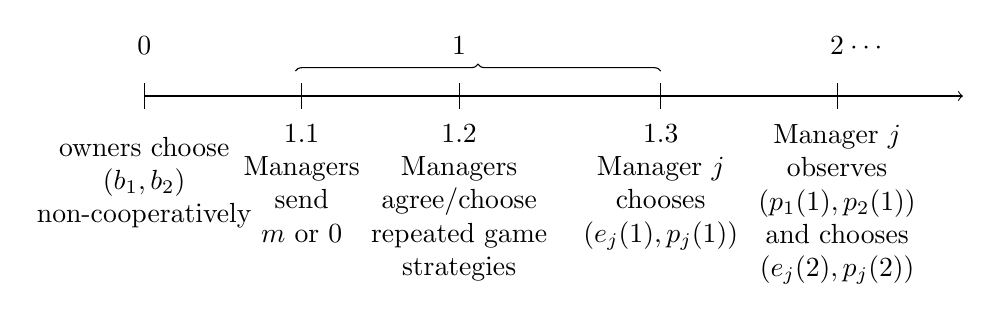
\begin{tikzpicture}[scale=0.8]
\draw[->] (0,0) -- (13,0);
\draw (0,-.2) -- (0, .2);
\draw (2.5,-.2) -- (2.5, .2);
\draw (5,-.2) -- (5, .2);
\draw (8.2,-.2) -- (8.2, .2);
\draw (11,-.2) -- (11, .2);
\node[align=center, below] at (0,-.5)
{owners choose\\
$(b_1,b_2)$\\
non-cooperatively};
\node[align=center, below] at (2.5,-.3)%
{1.1\\
Managers\\ send \\$m$ or $0$};
\node[align=center, below] at (5,-.3)%
{1.2\\
Managers\\agree/choose\\
repeated game\\strategies};
\node[align=center, below] at (8.2,-.3)%
{1.3\\Manager $j$\\
chooses\\
$(e_j(1),p_j(1))$};
\node[align=center, below] at (11,-.3)%
{Manager $j$\\
observes \\$(p_1(1),p_2(1))$\\
and chooses\\
$(e_j(2),p_j(2))$};
\node[align=left, above] at (0,.5)
{0};
\node[align=center, above] at (5,.5)%
{1};
\node[align=right, above] at (11,.5)%
{2};
\node[align=right, above] at (11.5,.5)%
{$\cdots$};
\draw[decoration={brace,raise=9pt},decorate]
  (2.4,0) -- node[above=10pt] {} (8.2,0); 
\end{tikzpicture}
\caption{Timing}
\label{fig:timing}
\end{figure}
%
\paragraph{Discussion.} Our assumption that managers can communicate only in the first period simplifies greatly the analysis, but is not restrictive. Indeed, under the maintained assumption that communication is necessary for coordination, if there is a first time $T\geq 2$ at which managers communicate, it must be true that for all $t\leq T-1$, managers play the static Nash action $p^c$. From time $T$ on, the strategic analysis is isomorphic to the analysis when $T=1$ (note that communication at $T\geq 2$ delays coordination, and managers would be better off communicating at time $1$.) The assumption is not restrictive either when we consider in Section \ref{sec:MS} the possibility of market signaling. Indeed, if there is a period of length $T-1$ during which managers do not communicate, either they use the static Nash actions during this period, in which case we are back to our analysis or they use market signaling in which case there is a first time $t_0<T$ at which the patient manager uses a different action than the myopic manager, and the analysis for $t\geq t_0$ is isomorphic to assuming that managers use market signaling in period $1$.

\paragraph{Communication.} After expressing their willingness to collude, the managers will sit at a bargaining table and decide on a course of action. At the time they negotiate, they have beliefs $q:=(q_{01},q_{\delta 1},q_{02},q_{\delta 2})$, about each other types, where $q_{ij}$ is the probability of manager of firm $j$ having type $i$. The course of action is a type-dependent Grimm-trigger repeated game strategy. The feasible set of decisions is the set of type-dependent Grimm-trigger repeated game strategies that are perfect Bayesian equilibria. 

Rather than using a specific bargaining process, we will use as a Nash cooperative bargaining concept in the spirit of the generalizations in  \cite{Harsanyi1972,Myerson1984,Weidner1992} to situations of asymmetry of information. We will focus on the solution where all the weight is put on the payoffs of patient types.\footnote{%
In the original solution of \cite{Harsanyi1972}, the weights on the type-payoffs coincide with the belief structure at the time of negotiation, see Appendix \ref{app:HS}. Our qualitative results do not depend on the particular weights that are used in the cooperative solution.} Hence, if $\sigma_{ij}$ is the repeated game strategy of type $i$ manager in firm $j$, the set of decisions is the set of strategies $\Sigma(q):=\left\{(\sigma_{01},\sigma_{\delta 1},\sigma_{02},\sigma_{\delta 2})\right\}$ that are perfect Bayesian equilibria given the belief structure $q$ at the time of negotiation. The threat point at the time of negotiation is to play each period the non-cooperative static equilibrium $\p^c$, hence an average payoff of $u^c(b):=b^2(\pi^c)^2/2$ in case of failure of bargaining. 

A Nash bargaining solution is a strategy $\sigma$ that maximizes the Nash product 
\[\left(U_{\delta 1}(\sigma,b_1;q)-u^c(b_1)\right)\left(U_{\delta 2}(\sigma,b_2;q)-u^c(b_2)\right),\]
 where $U_{\delta j}(\sigma,b_j;q)$ is the per-period expected payoff of type $\delta$ in firm $j$ when $\sigma$ is played and the manager has bonus $b_j$. As will become clear soon, because average payoffs are proportional to $b^2/2$, bonuses do not affect the Nash bargaining solution.

\subsection{Informative Communication Equilibrium}\label{sec:sep_eq}
We start our analysis by assuming that communication is perfectly informative about the managers' types, and that only patient types send a message. Along the equilibrium path, a manager who communicates believes that the other manager is patient only if she also sent a message. We first fix the levels of bonuses and analyze whether the outcome of coordination by the patient managers is such that the incentives for communication are consistent with separation. These incentive compatibility conditions induce lower and upper bounds on bonuses. We will then derive the equilibrium bonus levels set (non-cooperatively) by the owners.%For convenience, we will use the following notation.

\paragraph{Static outcome.} If the managers are known to be myopic, they play the static Nash equilibrium in all the periods. Given the bonus levels, static best responses satisfy:
\begin{equation}
e_j=b_j \pi(p_j,p_{-j})
\end{equation}
and
\begin{equation}
p_j=\arg\max_p b_j e_j \pi(p,p_{-j})-\frac{e_j^2}{2}.
\end{equation}
%
Hence, as long as $e_j$ is positive, the equilibrium strategies are $p_1=p_2=p^c$, where $p^c$ is independent of $e_j$ and $b_j$. We assume that $p^c$ is unique. Because $e_j^c=b_j\pi^c$, each manager gets utility \[u^c(b_j)=\frac{b_j^2 (\pi^c)^2}{2},\] while owners get utility $b_j(1-b_j)(\pi^c)^2$.

\paragraph{Collusive outcome.} After the communication stage, if both managers communicate, they negotiate on a grim-trigger strategy profile given their belief $q=(0,1,0,1)$. Because they assign a zero probability to facing a myopic manager, we can ignore the strategy of myopic managers, and restrict attention to the strategies of the patient managers. Feasible strategies for the patient managers $1$ and $2$ are collusive prices $\p^*=(p^*_1,p^*_2)$ and a reversal to $p^c$ if a collusive price has not been used in the past. The bargaining outcome is defined by the Nash cooperative solution. 

If at time $t$ the managers have an history of taking the collusive action $\p^*$, when manager of firm $j$ chooses $p_j(t)$ at period $t$, she will exert an effort that maximizes $b_je_j\pi(p_j(t),p^*_{-j})-\frac{e_j^2}{2}$, hence $e_j=b_j\pi(p_j(t),p^*_{-j})$ and the static payoff of the manager is $b_j^2\frac{\pi(p_j(t),p^*_{-j})^2}{2}$. Because the payoff from deviation is also proportional to $\frac{b_j^2}{2}$, a Grim-trigger strategy is part of an equilibrium if
%
\begin{equation}\label{E-sep}
\pi(p^*_j,p^*_{-j})^2\geq (1-\delta)(\pi(BR(\p^*),p^*_{-j})^2+\delta (\pi^c)^2.	
\end{equation}
%
A Grim-trigger strategy $\p^*$ is in the set of prices $Esep$ when condition \eqref{E-sep} holds. The Nash bargaining problem is then (we ignore the proportionality factor $\frac{b_1^2b_2^2}{4}$).
\begin{equation*}
\max_{(p_1,p_2)\in Esep} \prod_{j\in\{1,2\}} \left(\pi(p_j,p_{-j}))^2 -(\pi^c)^2\right),
\end{equation*}
%
By Assumption \ref{ass:patient}, the IC constraint is satisfied at $(p^M,p^M)$, and a necessary condition for optimality \emph{in the unconstrained problem} is that\footnote{%
Indeed, the first order condition for $p_j$ is  
$2\pi(p_j,p_{-j})\frac{\partial \pi(p_j,p_{-j})}{\partial p_j}(\pi(p_{-j},p_j)^2-(\pi^c)^2)+2\pi(p_{-j},p_j)\frac{\partial \pi(p_{-j},p_j)}{\partial p_j}(\pi(p_j,p_{-j})^2-(\pi^c)^2)=0$
and therefore, the sum of these conditions yields $\sum_{j=1}^2
(\pi(p_j,p_{-j})^2-(\pi^c)^2)\left(\pi(p_j,p_{-j})\frac{\partial \pi(p_{j},p_{-j})}{\partial p_j}+\pi(p_{-j},p_j)\frac{\partial \pi(p_{-j},p_j)}{\partial p_j}\right)=0$. If collusion is beneficial, $\pi(p_j,p_{-j})^2-(\pi^c)^2$ is positive for each $j=1,2$, and therefore, a necessary condition is that $\pi(p_j,p_{-j})\frac{\partial \pi(p_{j},p_{-j})}{\partial p_j}+\pi(p_{-j},p_j)\frac{\partial \pi(p_{-j},p_{j})}{\partial p_j}=0$ for each $j$.
}
\begin{align*}
\pi(p_j,p_{-j})\frac{\partial \pi(p_j,p_{-j})}{\partial p_j} + \pi(p_{-j},p_j)\frac{\partial \pi(p_{-j},p_j)}{\partial p_j}=0, \text{ for each $j=1,2$,}
\end{align*}
hence that $\p=(p^M,p^M)$ that maximizes the sum of the \emph{square} of the managers' payoffs. Hence, managers do not maximize the sum of profits.

The effort levels in this case are $e_j(t)=b_j\pi^M$ and the patient manager of firm $j$ gets average utility $U_{\delta j}^M=\frac{b_i^2{ (\pi^M)}^2}{2}$ along the equilibrium path.
%
\subsubsection*{Incentives to Separate}
Types separate -- that is types $\delta$ send a message and types $0$ do not send a message -- if a patient manager is willing to bear a fine $f$ by sending a message $m$ and being able to collude (with probability $\alpha$) if the other manager is patient rather than not sending a message and face competition:

\begin{equation}\tag{ICpatient}%\label{IC-type-delta}
\alpha \frac{b^2 (\pi^M)^2}{2} + (1-\alpha)  \frac{b^2 (\pi^c)^2}{2} - (1-\delta)f \geq \frac{b^2 (\pi^c)^2}{2}.
\end{equation}
%
Because a myopic manager can send a message and replicates the bargaining that a patient manager would do, a myopic manager must prefer to face competition rather than to deceive the patient manager from the other firm:
%
\begin{equation}\tag{ICmyopic}%\label{IC-type-0}
\frac{b^2 (\pi^c)^2}{2}  \geq \alpha \frac{b^2 (\pi(Br(p^M),p^M))^2}{2} + (1-\alpha) \frac{b^2 (\pi^c)^2}{2} - f.
\end{equation}
%

The main insight from this section is that there can be separation at the communication stage if the antitrust fines on managers lie in a non-trivial interval, with an upper bound increasing in the discount factor. Furthermore, for fines in this interval there exists an equilibrium of the game with imperfect information and communication that has the same outcome as under perfect information: there is collusion if, and only if, the two types are patient, and otherwise there is competition.

\begin{lemma}\label{lem:com}
The types can separate via communication in period $1$ if, and only if,
\begin{equation}\label{sep-interval-fines}
\underbrace{\frac{\alpha b_i^2}{2 } ((\pi(Br(p^M),p^M))^2-(\pi^c)^2)}_{\equiv \underline{f}(b_i,\alpha,\delta)}\leq f \leq \underbrace{\frac{\alpha b_i^2}{2 (1-\delta) } ((\pi^M)^2-(\pi^c)^2)}_{\equiv \overline{f}(b_i,\alpha,\delta)}
\end{equation}
\end{lemma}
%
Assumption \eqref{ass:patient} insures that the set of fines satisfying condition \eqref{sep-interval-fines} is non-empty. Hence when communication leads to fines, whenever $f$ belongs to the interval $[\underline{f}(b_i, \alpha,\delta),\overline{f}(b_i, \alpha,\delta)]$, there exists an equilibrium of the game with communication that replicates the perfect information situation. That is, when the two types are patient, the outcome is $(p^M,p^M)$ while when one of the types is myopic the outcome is the short run outcome $(p^c,p^c)$. This proves the following proposition.
%
\begin{proposition}\label{prop:com}
There exists a non-empty interval $[\underline f(b_i, \alpha,\delta),\overline f(b_i, \alpha,\delta)]$ such that whenever $f$ belongs to this interval, there exists an equilibrium strategy of the game with imperfect information and costly communication that leads to the same market outcomes as the respective games of perfect information.
\end{proposition}
%
The equilibrium utility of a patient manager is  $\frac{b_i^2}{2} \left(\alpha (\pi^M)^2+(1-\alpha)(\pi^c)^2\right)-(1-\delta)f$, and a higher value of the fine in the interval of Proposition \ref{prop:com} decreases the payoff to the collusive types but does not affect the level of prices in the market: the fine neither deters collusion nor makes collusion less stable.

\begin{corollary}\label{cor:sep_bonuses}
Given the individual fines $f$, the types can separate via communication in period 1, if and only if the bonuses are in the following interval:
\begin{equation}\label{interval-bonuses}
\beta^{sep}_\delta(f) \equiv \sqrt{ \frac{2 (1-\delta)  f}{\alpha ((\pi^M)^2-(\pi^c)^2)} } \leq b \leq \sqrt{ \frac{2  f}{\alpha ((\pi(Br(p^M),p^M))^2-(\pi^c)^2)} }\equiv \beta^{sep}_0(f).
\end{equation}
The left inequality is the incentive compatibility of patient managers who should communicate and the right inequality is the incentive compatibility of myopic managers who should not communicate.
\end{corollary}
%
In Example \ref{ex1}, where the parameter values are $\gamma=1/2$, $\alpha=2/3$, and $\delta=8/10$, there can be separation of types through direct communication if, and only if, the bonuses are in the region delimited by the red and blue lines in Figure \ref{fig:sep_IC_bonuses}. The horizontal axes in the figure is the level of individual fines imposed to the managers as a percentage of one period collusive profit of the firm.

But owners have a direct stake in whether there is communication: they may benefit from it as collusion yields higher profits, but they also bear the antitrust cost of the expected fine $F$. The Corollary \ref{cor:sep_bonuses} suggests that the owners can use the bonus to indirectly control communication, and we analyze next when they will have such an incentive.
%
\begin{figure}[ht]
\centering
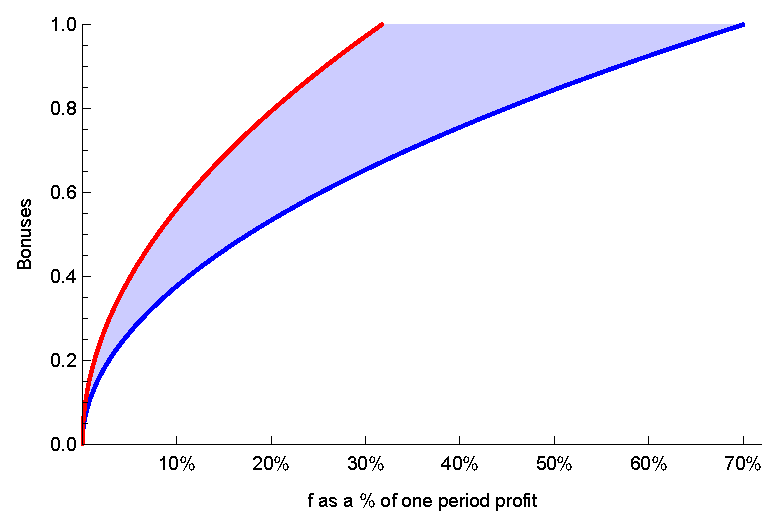
\includegraphics[scale=0.8]{Plots/Bertrand_sep_IC_bonuses.eps}
\caption{IC conditions in example \ref{ex1}\\ (Red: IC condition for type $0$. Blue: IC condition for type $\delta$).}\label{fig:sep_IC_bonuses}
\end{figure}

\subsubsection*{Owners' Choices of Bonuses.} 
Owners who want to induce separation in communication will choose $b$ to maximize
\begin{align}\label{prog:owners}
\max_{b}&\; b (1-b) \big[\alpha^2 (\pi^M)^2 + (1-\alpha^2) (\pi^c)^2\big]- \alpha (1-\delta)F\\
\text{s.t. }&b\in[\beta^{sep}_\delta(f),\beta^{sep}_0(f)].\notag
\end{align}
%
Without the constraint, the optimal level of the bonuses would be $b=1/2$. However, $b=1/2$ is consistent with the incentive compatibility conditions \eqref{interval-bonuses} only for an intermediate range of fines. When the fine faced by managers is outside this range, the optimal bonus is an increasing function of $f$, hence lower than $1/2$ for low fines and greater than $1/2$ for high fines.
\begin{equation}\label{bonuses-sep}
b^{sep}(f) = 
\begin{cases}
\beta^{sep}_0(f) & \text{ if }\beta^{sep}_0(f) \leq 1/2 \\         
1/2 & \text{ if }\beta^{sep}_\delta(f) \leq 1/2 \leq \beta^{sep}_0(f) \\
\beta^{sep}_\delta(f) & \text{ if }\beta^{sep}_\delta(f)>1/2.
\end{cases}
\end{equation}
Solid lines in Figure \ref{fig:bonuses} depicts these bonus levels in Example \ref{ex1}.

\begin{figure}[ht]
\centering
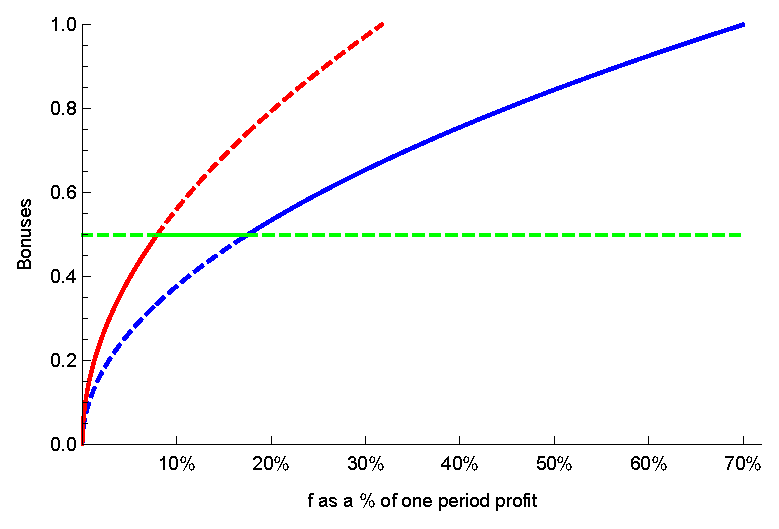
\includegraphics[scale=0.8]{Plots/Bertrand_bonuses_diff.eps}
\caption{Bonus levels consistent with a separating equilibrium in Example \ref{ex1}.}\label{fig:bonuses}
\end{figure}

Owners have an expected expected profit
\begin{equation}\label{eq:sep_profit}
V^{sep}(F,f)=b^{sep}(f)(1-b^{sep}(f)) \left[ \alpha^2 (\pi^M)^2 + (1-\alpha^2) (\pi^c)^2 \right] - \alpha (1-\delta)F.
\end{equation}
%
Separation is an equilibrium if an owner does not want to discourage it by setting a bonus outside the range defined in Corollary \ref{cor:sep_bonuses}. If $b<\beta^{sep}_\delta(f)$, no type will communicate and the owner saves $\alpha F$; if $b>\beta^{sep}_0(f)$, both types will communicate and the owner pays an additional fine $(1-\alpha)F$. As we show the owner does not want to lower or increase the bonus outside the separating regions when the fine is neither too low nor too high. Indeed, a deviation by an owner to a bonus outside the range $[\underline b,\overline b$] will prevent separation (when the owner of the firm uses bonus $b{sep}(f)$).
%
\paragraph{Deviation to  $b<\beta^{sep}_\delta(f)$,}  In this case, managers are not willing to communicate and the owner has expected payoff of $b(1-b)(\pi^c)^2$, which is smaller than $V^{sep}(F,f)$ if $F$ is smaller than a bound $\overline F^{sep}(f)$. The exact value of the bound depends on the regime that defines $b^{sep}(f)$. The owner's best deviation is to choose $b^{d1}(f)=1/2$ if $\beta^{sep}_\delta(f)>1/2$ and to choose $b^{d1}(f)=\beta^{sep}_\delta(f)$ when $\beta^{sep}_\delta(f)\leq 1/2$.\footnote{In the latter case, $b^{sep}(f)$ is equal to $min(1/2,\beta^{sep}_0(f))$, and therefore, while the patient manager is indifferent between communicating and not at $\beta^{sep}_\delta(f)$, we can assume that she will not communicate when the owner sets the out-of-equilibrium bonus $\beta^{sep}_\delta(f)$.} The supremum of the profit an owner can obtain by choosing such a deviation is attained at 
%
\[
V^{d1}(F,f):=b^{d1}(f)(1-b^{d1}(f)) \big[(\pi^c)^2\big],
\]
and this must be smaller than $V^{sep}(f,F)$, implying an upper bound $\overline F^{sep}(f)$ on $F$.

\paragraph{Deviation to $b>\beta^{sep}_0(f)$.} Then myopic managers also want to communicate (but the other manager believes that she is facing a patient manager if there is communication). The owner best deviation is to choose set $b^{d2}(f)=1/2$ if $\beta^{sep}_0(f)\leq 1/2$ and $b^{d2}(f)=\beta^{sep}_0(f)$ when $\beta^{sep}_0(f)> 1/2$.\footnote{As in the previous case, if $\beta^{sep}_0(f)> 1/2$, $b^{sep}(f)=\max(1/2,\beta^{sep}_\delta(f)$ and therefore, we can assume that the manager will not communicated for the out-of-equilibrium bonus $\beta^{sep}_0(f)$.}  Hence the supremum of the profit an owner can achieve when both types communicate is
%
\begin{equation*}%\label{eq:pool_profit}
\begin{split}
V^{d2}(F,f):=b^{d2}(f)(1-b^{d2}(f))& \Big[\alpha^2 (\pi^M)^2+\alpha(1-\alpha)(1-\delta)(\pi(Br(p^M),p^M))^2\\
&+(1-\alpha)(1+\alpha \delta) (\pi^c)^2\Big] - (1-\delta)F.
\end{split}
\end{equation*}
%
which is smaller than $V^{sep}(f,F)$ if $F$ is greater than a lower bound $\underline F^{sep}(f)$.
%
\begin{proposition}\label{prop:separation-owners-managers}
It is an equilibrium for the owners to induce separation of types through direct communication if, and only if, they both face a fine in the interval $[\underline{F}{sep}(f),\overline{F}{sep}(f)]$.  
\end{proposition}
%
If the owners want to induce separation, the optimal bonus maximizes the product $b(1-b)$ subject to the incentive compatibility constraint \eqref{interval-bonuses}. There is, therefore, a distortion with respect to the unconstrained optimum $b=1/2$ only when the level of fine $f$ is outside of the interval $[\underline b^{-1}(1/2),\overline b^{-1}(1/2)]$. In these cases, the owners choose the level of bonus in order to induce separation and could be deemed co-responsible for the collusive outcome and direct communication between their managers.

Using the same parametric values as before in Example \ref{ex1}, the area shown in Figure \ref{fig:fines} illustrates Proposition \ref{prop:separation-owners-managers}: it delineates the values of the fines $F,f$ for which separation of the types can be an equilibrium. For convenience we have transformed the expected fines $F$ and $f$ into percentages of realized profits assuming that $b=1/2$ (as $F,f$ change, the bonus level will change and the profit of the owners will be in general lower than when $b=1/2$). If the sum of the expected fines is large, the owners will avoid collusion. If the sum of the fines is small, then separation is not an equilibrium and in this case, it is not optimal for the owners to distort the bonus away from $1/2$. The gray lines depict the cases in which the sum of the fines equal to a given percentage of firm's profit and the allocation of fines between the owner and the manager plays an important role. For large set of fines, if one of the two parties has to pay most of the total expected fine, then the separation of types is not possible through communication. Moreover, if the level of total \textit{expected} fines increases (beyond 75\%) then separation is less likely to happen.
\begin{figure}[ht]
\centering
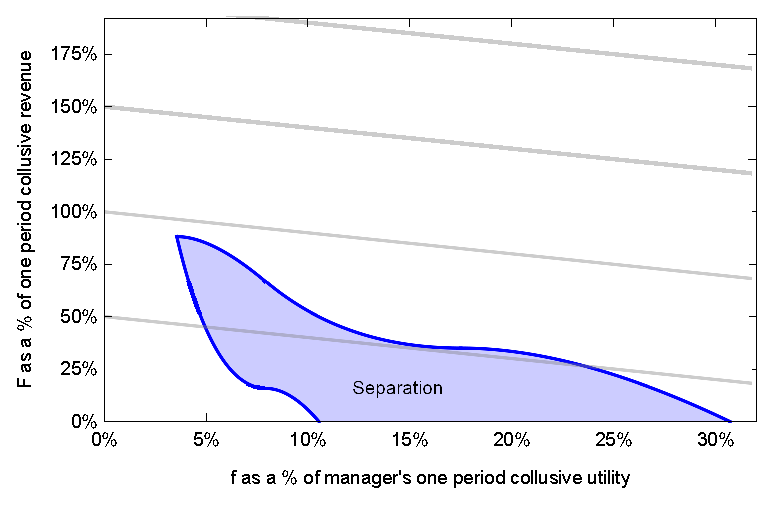
\includegraphics[scale=0.8]{Plots/Bertrand_sep_f_F.eps}
\caption{Owner-optimal induced communication strategy of the manager given $f,F$.}\label{fig:fines}
\end{figure}
%
As already noted, $F$ and $f$ are expected levels of fines rather than absolute values. By most estimates, the probability of detection of a cartel is between $12\%$ and $17\%$, so a $10\%$ of turnover expected fine means an actual fine in case of detection between $60\%$ and $80\%$ of the firm's total profits, which is well above the actual levels of fines. This suggests that the set of fines consistent with having separation of types during communication is a non-trivial set, at least in the parametric Example \ref{ex1}. 

In general, separation is not an equilibrium if there are only corporate fines: fines on managers facilitate informative communication and collusion. Even if separation of types is not possible, owners may value the managers' communication in order to coordinate on collusive strategies. In this case, the managers do not reveal their types and the negotiation happens under imperfect information. We turn to this "pooling" case now and show that the lack of individual fines on managers leads to more communication between the managers and to the pooling equilibrium.

\subsection{Pooling Equilibrium}
\subsubsection*{Manager's problem.}
All types send messages and therefore during negotiation on a grim-trigger strategy, patient players anticipate that the myopic managers will undercut the collusive price. This will limit the level of collusive prices; in general, below the level that maximizes the sum of the patient managers' payoffs. For simplicity, we restrict attention to type-symmetric equilibria. 
%
\paragraph{Incentive compatibility.} During negotiation, managers agree on a repeated game strategy for each type  $\sigma=(\sigma_{01},\sigma_{\delta 1},\sigma_{02},\sigma_{\delta 2})$. Patient managers use a `double'' Grimm-trigger strategy: the first period history triggers either the competitive equilibrium or a collusive Grimm-trigger strategy:
\begin{itemize}
    \item At $t=1$, play $p^*>p^c$.
    \item At $t\geq 2$, play the Grimm trigger strategy with collusive price $p^{**}$ and reversal to $p^c$ only if both managers set price $p^*$ in period $1$; otherwise play $p^c$.
\end{itemize}
%
Let $p^d$ be the first period price that myopic managers should use, the superscript $d$ stands for ``deviation''. Given the strategy of patient managers, a myopic manager $0j$ faces a manager of type $\delta$ with probability $\alpha$ who plays $p^*$ and faces a manger of type $0$ with probability $1-\alpha$ who plays $p^d$. Therefore, $\sigma_{0j}$ is part of a perfect Bayesian equilibrium only if\footnote{Note that, the optimal effort level of the myopic player is $e^d = b (\alpha \pi(p,p^*) + (1-\alpha) \pi(p,p^d))$ and the myopic player maximizes $\frac{b^2}{2} (\alpha \pi(p,p^*) + (1-\alpha) \pi(p,p^d))^2$.}
%
\begin{equation}\label{pool:IC0}
\sigma_{0j}(\emptyset)=p^d \in \arg\max_{p} \alpha \pi(p,p^*)+(1-\alpha)\pi(p,p^d).
\end{equation}
%
At times $t\geq 2$, if the history is $h^*(t)=\left((p^*,p^*),(p^{**},p^{**})^{t-2}\right)$, patient players are expected to play 
$p^{**}$ while myopic players are expected to play $\sigma_{0j}(h^*(t))$. Clearly, $h^*(t)$ is an out-of-equilibrium history for myopic managers. In this case, a myopic manager believes that the other manager is patient since a myopic manager is expected to play $p^d\neq p^*$ in the first period, and therefore,
\[
\sigma_{0j}(h^*(t))\in \arg\max_{p} \pi(p,p^{**})
\]
Myopic managers' type will be revealed at time $2$, and therefore, they are expected to play $p^c$ after the second period. If the history is not $h^*(t)$, patient managers play $p^c$ and therefore myopic managers must play $p^c$ in a perfect Bayesian equilibrium. Given these strategies of myopic managers, the double Grimm-trigger strategy of patient managers is a best response at any history, and managers will negotiate over the set of such strategy profiles. 

For a patient player $\delta j$, playing $p^*$, in the first period, yields an expected payoff
%
\[
\frac{b_j^2}{2}\left((1-\delta)[\alpha \pi(p^*,p^*)+(1-\alpha)\pi(p^{*},p^d)]^2 + \delta [ \alpha (\pi(p^{**},p^{**}))^2 + (1-\alpha) (\pi^c)^2]\right) - (1-\delta) f.
\]
If the patient player deviates from $p^*$, she will face a continuation payoff of $\pi^c$. Her best deviation is the same as the equilibrium action of a myopic manager, that is $p^d$, and her maximum payoff from deviation is
%
\[
\frac{b_j^2}{2}\left((1-\delta)[\alpha \pi(p^d,p^*)+ (1-\alpha) \pi(p^{d},p^d)]^2 + \delta (\pi^c)^2\right) - (1-\delta) f,
\]
implying that the patient player does not deviate when
\begin{equation}
  \begin{split}\label{pool:ICdelta}
    (1-\delta)[\alpha \pi(p^*,p^*)+(1-\alpha)\pi(p^{*},p^d)]^2 + \delta \alpha (\pi(p^{**},p^{**}))^2 \geq \\
(1-\delta)[\alpha \pi(p^d,p^*)+ (1-\alpha) \pi(p^{d},p^d)]^2 + \delta \alpha (\pi^c)^2
  \end{split}
\end{equation}
%
This condition may fail to be satisfied at $p^*=p^M$. Nevertheless, we note that as $p^*$ decreases to $ p^c$ the deviation $p^d$ decreases to $p^c$ in \eqref{pool:IC0} and therefore \eqref{pool:ICdelta} is satisfied. Therefore, there exists $p^*>p^c$ and $p^d$ satisfying both \eqref{pool:IC0} and \eqref{pool:ICdelta}. 
%%%%%
%   
% Nash nargaining in pooling  %             
%    
%%%%%
\paragraph{Nash bargaining.} We define the set $Epool$ of strategies $\sigma$ satisfying conditions \eqref{pool:IC0} and \eqref{pool:ICdelta}. For such strategies, patient managers choose effort levels $e_j=b_j  [\alpha \pi(p^*,p^*) +(1-\alpha) \pi(p^*,p^d]$ in the first period. From period $2$ on, patient managers have an average continuation value $\frac{b_j^2}{2}(\pi(p^{**},p^{**})^2$ if first period prices are $\p^*$ or $\frac{b_j^2}{2}(\pi^c)^2$ if first period prices are different from $\p^*$. Taking into account the optimal effort levels, the expected discounted value of patient managers for agreements in $Epool$ is equal to $b_j^2 U^{pool}(\sigma)/2$, where 
%
\begin{equation*}
  \begin{split}
    U^{pool}(\sigma):= &(1-\delta)\left(\alpha\pi(p^*,p^*)+(1-\alpha)\pi(p^*,p^d)\right)^2\\
&+\delta\left(\alpha\left(\pi(p^{**},p^{**}\right)^2+(1-\alpha)(\pi^c)^2\right)
  \end{split}
\end{equation*}
%
and therefore, Nash bargaining selects a strategy $\sigma$ solving
%
\begin{equation}\label{Nash:pool}
     \max_{\sigma\in Epool} \Big(U^{pool}(\sigma)-(\pi^c)^2\Big)^2
\end{equation}

%
It is clear that $p^{**}=p^M$ maximizes $U^{pool}(\sigma)$, and makes the incentive condition \eqref{pool:ICdelta} easier to satisfy. Therefore, it is sufficient to define the first period price $p^*$ (as $p^d$ is given by \eqref{pool:IC0}.)
%
\begin{example}
	In the environment of Example \ref{ex1}, $p^M=1$. Focusing on symmetric strategies, $Epool\approx[0.259,1.1275]$ and the solution to \eqref{Nash:pool} is $p^*=6/7$. This price is lower than the collusive price under perfect information $p^M$, illustrating the cost that imperfect information about the other manager's willingness to collude impose on first period collusion. 
\end{example}
%
\paragraph{Incentives to communicate in a pooling equilibrium.} 
A patient manager sends a message if 
\begin{equation}\label{ICpatientpool}
\begin{split}
	\frac{b^2_j}{2}\Big[(1-\delta) \big( \alpha &\pi(p^*,p^*) + (1-\alpha) \pi(p^*,p^d) \big)^2 \\
	&+ \delta (\alpha(\pi^M)^2  + (1-\alpha) (\pi^c)^2)\Big]-(1-\delta)f \geq \frac{b^2_j}{2} (\pi^c)^2 \text{.} 
\end{split}
\end{equation}
%
A myopic manager is also willing to send a message if
\begin{equation}\tag{ICmyopicpool}\label{ICmyopicpool}
 \begin{split}
 	\frac{b^2_j}{2} \left[\alpha \pi(p^d,p^*)+(1-\alpha)\pi(p^d,p^d)\right]^2 -f \geq \frac{b^2_j}{2} (\pi^c)^2 \text{.}
 \end{split}
\end{equation}
It should be clear that condition \eqref{ICmyopicpool} implies condition \eqref{ICpatientpool}. Let $f^{pool}_0(b)$ be the value of $f$ that binds the incentive compatibility condition \eqref{ICmyopicpool} of myopic types.
%
\begin{lemma}\label{lem:com_pooling}
All types communicating is an equilibrium in period $1$ if, and only if, $f$ is inferior $f^{pool}_0(b)$.
\end{lemma}
%
Alternatively, fixing $f$, the IC condition \eqref{ICmyopicpool} binds at a level $\beta^{pool}_0(f)$ that is superior to the value $\beta^{pool}_\delta(f)$ for which condition \eqref{ICpatientpool} binds. 

\begin{corollary}\label{cor:pool_bonuses}
Given an individual fine $f$, both types communicate in period $1$ if, and only if, the bonuses are higher than the bonus level $\beta^{pool}_0(f)$ at which the myopic types are indifferent between communicating and not.
\end{corollary}

Figure \ref{fig:pool_IC_bonuses} illustrates the IC conditions and the region of bonus levels $b\geq\beta^{pool}_0(f)$ consistent with communication and pooling in the first period in the environment of Example \ref{ex1}.
%
\begin{figure}[h!]
\centering
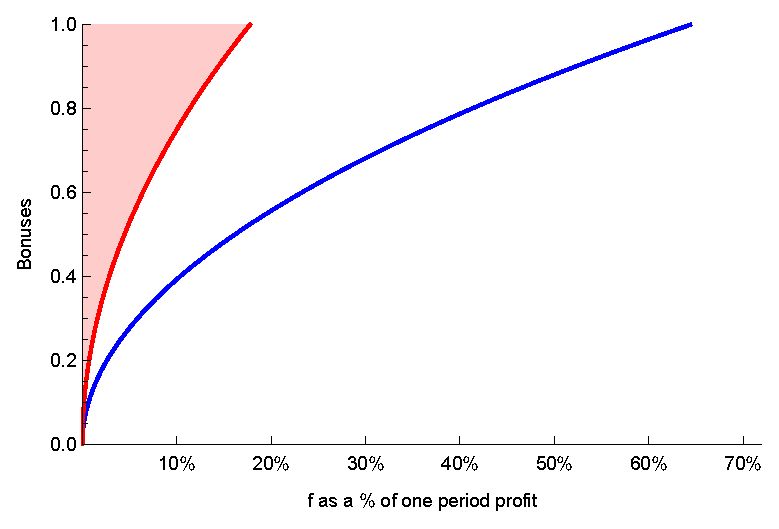
\includegraphics[scale=0.8]{Plots/Bertrand_bonuses_diff_bonus_pool.eps}
\caption{IC conditions in Bertrand example (red: $f^{0}_{pool}(b_i,\alpha,\delta)$ -- IC condition for type $0$, blue: $f^{pool}_\delta(b)$ -- IC condition for type $\delta$).}\label{fig:pool_IC_bonuses}
\end{figure}

\subsubsection*{Owner's problem.} 

Corollary \ref{cor:pool_bonuses} gives us the necessary condition for the pooling equilibrium for the managers. In this subsection, we analyze when it is optimal for each owner to give the right incentives to its manager to communicate independently of her type.

As in the separating equilibrium case, without the incentive constraints for communication, the optimal level of the bonuses is $1/2$. When $\beta^{pool}_0(f)$ is lower than $1/2$, it is optimal for the owner to choose the bonus level $1/2$ in the pooling equilibrium. Therefore, the optimal bonus levels consistent with pooling is
%\footnote{
%The profit of owners for bonus $b$  is given by
%\begin{align*}
%(1-b)b & \left[ \alpha \left( (\alpha \pi(p^*,p^*)+(1-\alpha)\pi(p^*,\sa))^2 +\frac{\delta}{1-\delta} \left(\alpha (\pi^M)^2 + (1-\alpha) (\pi^c)^2\right) \right)\right.\\
%&\left. + (1-\alpha) \left( (\alpha \pi(\sa,p^*)+(1-\alpha)\pi(\sa,\sa))^2 +\frac{\delta}{1-\delta} (\pi^c)^2 \right) \right] - F \text{.} \notag
%\end{align*}}
\begin{equation}\label{bonuses-pooling}
b^{pool}(f) = 
\begin{cases}
1/2 & \text{ if }\beta^{pool}_0(f) \leq  1/2 \\
\beta^{pool}_0(f) & \text{ if }\beta^{pool}_0(f)>1/2.
\end{cases}
\end{equation}
The green line in Figure \ref{fig:optimal_bonuses_pooling} represents the efficient bonus for owners and therefore using Figure \ref{fig:pool_IC_bonuses}, owners want to use bonuses corresponding to the upper-contour of the green and red line (the minimum bonus consistent with myopic managers willing to communicate for a given $f$).
%
\begin{figure}[h!]
\centering
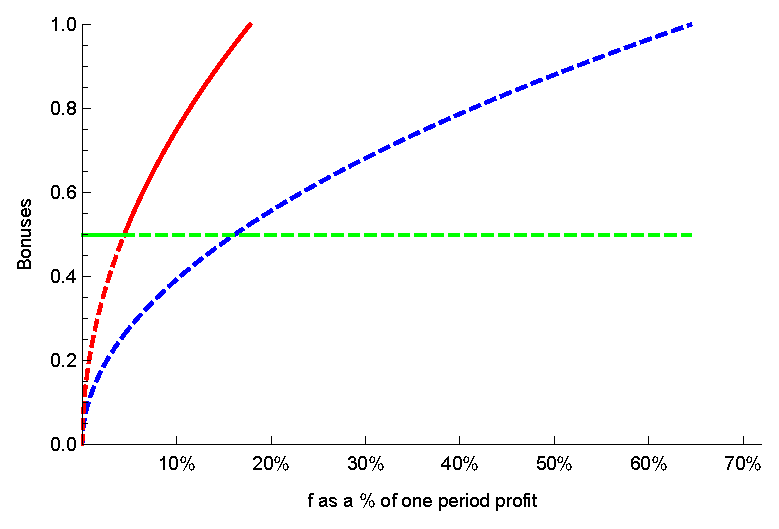
\includegraphics[scale=0.8]{Plots/Bertrand_bonuses_diff_bonus_pool2.eps}
\caption{Bonus levels in pooling equilibrium (solid curve)\\
Red: IC of myopic managers: Blue: IC of patient managers\\
Green: efficient bonus.}\label{fig:optimal_bonuses_pooling}
\end{figure}

Pooling is an equilibrium if the owners do not want to prevent communication. 
\paragraph{First type of deviation.} 
The owner of a firm can deviate by setting a bonus in the interval  $(\beta^{pool}_\delta(f),\beta^{pool}_0(f))$. In this case, only type $\delta$ will communicate and the expected payoff of the owner will be
\begin{align}\label{pool-owners-first-dev}
(1-b)b \Big\{ \alpha \Big[
(1-\delta)[(\alpha \pi(p^*,p^*)&+(1-\alpha)\pi(p^*,p^d)\big]^2 +\delta (\pi^M)^2\Big]\\
 &+ (1-\alpha) (\pi^c)^2\Big\} - \alpha (1-\delta)F \text{.} \notag
\end{align}
The best deviation in this first case is\footnote{\label{ft:rmk-discrete}%
The deviation assumes that the manager will not communicate when she is indifferent between communicating. Alternatively, because we want to show that there \emph{does not exist} a deviation by owners, rather than proving that there is a ``best'' deviation, our arguments apply if we consider a ``slightly'' lower bonus than what is in \eqref{bonuses-pooling}. %
}
\begin{equation}\label{[pool_dev_1}
b^{d1}(f) = 
\begin{cases}
\beta^{pool}_0(f) & \text{ if }\beta^{pool}_0(f) \leq  1/2 \\         
1/2 & \text{ if }\beta^{pool}_\delta(f) <  1/2 <  \beta^{pool}_0(f) \\
\beta^{pool}_\delta(f) & \text{ if }\beta^{pool}_\delta(f)\geq1/2.
\end{cases}
\end{equation}
In this deviation, the owner saves $(1-\alpha)F$, but loses the expected deviation profit from type $0$. If we compare the expected profit from this deviation with the expected profit of the owner from playing pooling, we get a first condition for the corporate fines $F<{F}_{pool}^1(f)$ to be consistent with pooling.

\paragraph{Second type of deviation.} A second deviation, is when the owners of a firm set a bonus lower than $\beta^{pool}_{\delta}(f)$. In this case, no type communicates and the owners' payoff is given by
\begin{equation*}
    b(1-b)(\pi^c)^2.
\end{equation*}
The best deviation in this case is
\begin{equation}\label{pool-dev_2}
b^{d2}(f) = 
\begin{cases}
\beta^{pool}_\delta(f) & \text{ if }\beta^{pool}_\delta(f)  \leq  1/2 \\
1/2 & \text{ if }\beta^{pool}_\delta(f)>1/2.
\end{cases}
\end{equation}
In this deviation,\footnote{%
Same remark as in footnote \ref{ft:rmk-discrete}.} the owner saves the fine $F$, but loses the expected gains after communication. From the comparison of the expected profits of the owners from this deviation and the pooling strategy, we can get the second condition for the corporate fines $F<{F}^{d2}_{pool}$. The minimum of these fines is $$\overline{F}^{pool}(f):=\min\{{F}^{d1}_{pool}(f), F^{d2}_{pool}(f)\}.$$

\begin{proposition}\label{prop:pooling-owners-managers}
It is an equilibrium for the owners to induce pooling if, and only if, they face a fine $F<\overline{F}^{pool}(f)$.
\end{proposition}

Figure \ref{fig:fines_pool} shows the area of the fines in which pooling is an equilibrium in Example \ref{ex1}. Pooling is an equilibrium for a wide range of corporate fines. Figure \ref{fig:fines_pool_sep} combines the previous figures and shows the regions where fines are consistent with either a separating or a pooling equilibria. Elsewhere the only equilibrium is competition. 

\begin{figure}
\centering
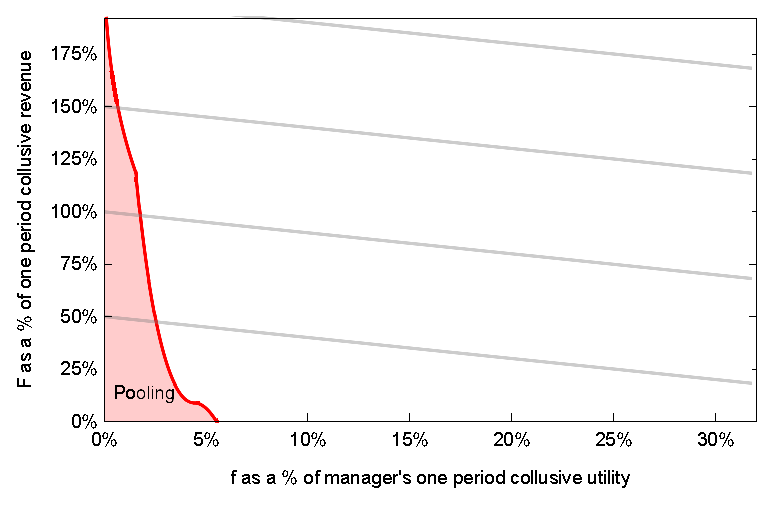
\includegraphics[scale=0.8]{Plots/Bertrand_com_f_F_Pool.eps}
\caption{Owner-optimal induced pooling strategy of the manager given $F,d$.}\label{fig:fines_pool}
\end{figure}

\begin{figure}
\centering
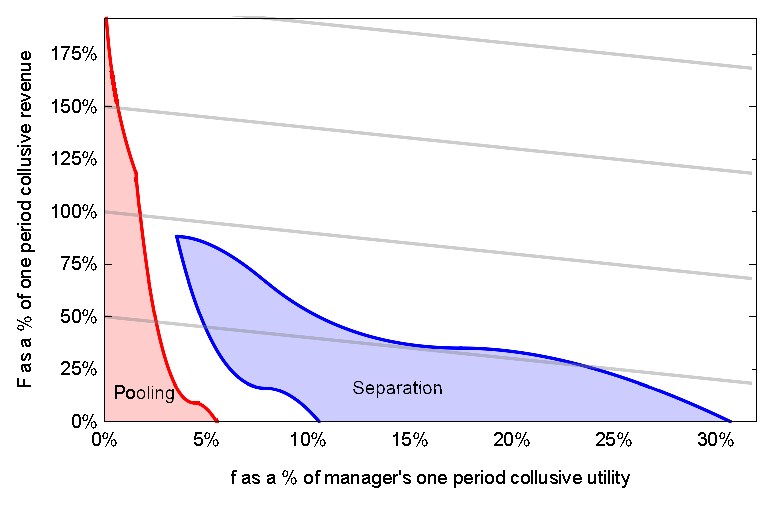
\includegraphics[scale=0.8]{Plots/Bertrand_com_f_F_SepvsPool.eps}
\caption{Separating vs pooling equilibrium.}\label{fig:fines_pool_sep}
\end{figure}

 
If collusion requires that that managers communicate and agree on a course of action, owners will want to induce this communication, even at the cost of deviating from the optimal bonus. We illustrate this in Figure \ref{fig:cs}.%\footnote{Figure \ref{fig:bonuses} indicates, for a given value of $F$, the bonuses required to induce informative communication (separation) as a function of the fine faced by managers and figure \ref{fig:fines} when owners will want to induce separation as a function of the relative fines $(F,f)$. The same information is available in figures  \ref{fig:bonuses_pooling} and \ref{fig:fines_pool} for non-informative (pooling) communication.}

\begin{figure}[h!]
\centering
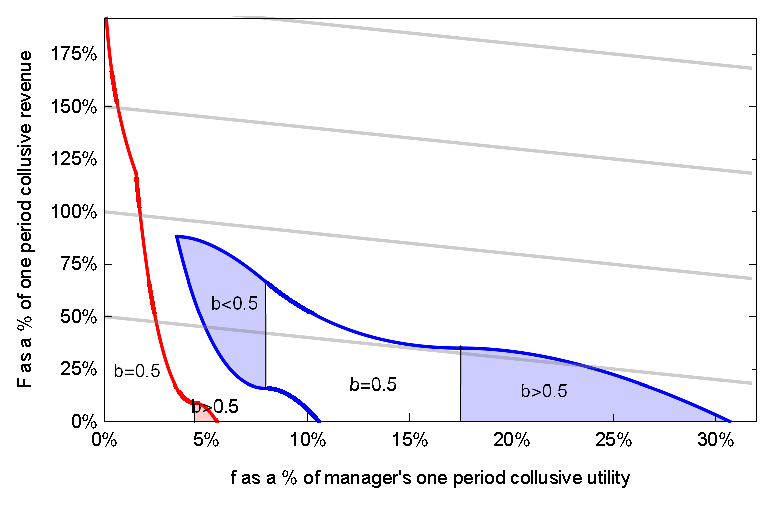
\includegraphics[scale=0.9]{Plots/Bertrand_bonuses_f_F.eps}
\caption{Bonuses and communication equilibria.}\label{fig:cs}
\end{figure}
%
In the separating region, there can be two types of distortions from the first-best bonus $b=1/2$, which correspond to two ways managers can be compensated for the antitrust fines they will bear if they communicate their willingness to collude. If the expected fine is low, the increased profit due to collusion is sufficient as a compensation to patient managers. In this case, the bonuses are lower, as myopic managers would have an incentive to communicate if the bonus stays at the efficient level. If, however the expected antitrust fine is large, the increase in profit after collusion is not sufficient to compensate for the fine and the bonus of patient managers must increase beyond the efficient level (myopic managers are incentive compatible because their communication constraint is more difficult to satisfy than that of patient managers).

In the pooling region, there is no need to depart from the efficient bonus unless the managerial fine is high and the owner's fine is low: the first condition is to insure that myopic managers want to communicate, the later to insure that the benefit of inducing pooling by increasing slightly the bonus is not smaller than the expected antitrust fine. At least in the specification of Example \ref{ex1}, that region is small.

The disconnectedness of the two regions of communication equilibria is due to the discontinuities in behaviors of owners and managers for small changes in $(F,f)$ when the incentive constraints bind. 

For instance, consider the red curve indicating the binding incentive constraint for pooling. If fixing $f$ we increase $F$, owners are no longer willing to implement a pooling equilibrium. As reflected in Propositions \ref{prop:com} and \ref{prop:pooling-owners-managers}, $\overline F^{pool}(f)$ is inferior to $\underline{F}^{sep}(f)$. $\overline F^{pool}(f)$ is the upper bound of the fine which is compatible with the owners inducing communication for myopic types in the pooling equilibrium. While, $\underline{F}^{sep}(f)$ is the lower bound of the fines which makes the owners to prevent communication for the myopic types. Note that, owners can gain more from the communication of myopic players when the other manager believes that only patient managers communicate. Therefore, the lower bound of the fines in the separating equilibrium, $\underline{F}^{sep}(f)$, is larger than the upper bound of the fines in the pooling equilibrium.

\section{Tacit Coordination and Market Signaling}\label{sec:MS}
Even without direct communication, past actions may be used by managers to signal their types (as in parallel pricing or price leadership). As summarized in section \ref{lit:tacit}, whether collusion can be sustained in the absence of direct communication is a subject of debate in the literature. Nevertheless, when managers have private information about their willingness to collude, ``market signaling'' seems an alternative to direct communication; it may be less effective to transmit information but may avoid antitrust fines.

Like in the pooling equilibrium under communication, in the first period, a myopic manager can free ride on the high price that a patient manager sets to signal her type, implying that the patient manager has an opportunity cost of setting a too high price in the first period. However, because there are no fines, the only relevant incentive constraints relate to first period prices and are reflected in the set $Epool$ of first period prices $p^*$ for the patient managers and $p^d$ for the myopic managers. As the owners cannot influence the managers' incentives to collude, they will set the bonus levels which optimize the effort levels, \textit{i.e.}, $b_i=1/2$.

It is immediate that owners are better off in a market signaling equilibrium than in a pooling equilibrium under direct communication. Indeed, the owners' expected payoff in the market signaling equilibrium is equal to their payoffs from the pooling equilibrium when the bonuses are equal to $1/2$ and $F=0$ (we have assumed that tacit collusion does not yield to fines, but the logic is the same as long as the fine is lower than under explicit communication). As $1/2$ is the efficient level of bonuses, in the pooling equilibrium, any deviation from $1/2$ decreases owners' expected payoffs and any $F>0$ decreases their expected payoffs even more. 

However, owners may prefer a separating equilibrium to market signalling if there is a high probability that managers are patient. But there is a cost to such transparency. Indeed, with separation of types, only patient managers coordinate on the collusive outcome in the first period, and there is no collusion as soon as one manager is myopic. By contrast, with market signaling, there is always the possibility of collusion, but at a lower collusive price in the first period for patient managers ($p^*  p^M$) and a larger price by myopic managers $p^d>p^c$. Hence, if there is a probability of having myopic managers, market signalling may dominate informative communication for owners. This is the case in the environment of Example \ref{ex1}.\footnote{%
It can be shown that when market signalling is possible, patient managers prefer direct communication over market signaling only if $b>1/2$. In all other cases, both the managers and the owners prefer market signaling to communication.}

\begin{corollary}
In Example \ref{ex1}, if market signalling is possible and not illegal, expected average prices in the industry may be higher than under the separating equilibrium with communication and fines.
\end{corollary}
%
Consumers face high prices under both market signalling and explicit communication, but with informative communication, they may face lower expected prices in the first period. Indeed, because the antitrust fine helps signalling when there is direct communication, consumers face high prices only if both managers are patient; in the other cases the outcome is the static Bertrand. By contrast, with market signalling, the short-term managers free ride on the long-term managers. It follows that long-term managers set a lower price than the monopoly price but short-term managers set a higher price than the static Bertrand quantity. Therefore, the expected price may be greater -- and consumer surplus may be lower -- than in the separating equilibrium, but this effect seems small in simulations. 

\begin{example}
For the demand functions $q_i=1-p_i+\gamma p_j$, the consumer surplus is given by\footnote{%
In our model, bonuses do not affect the consumer surplus and the continuation values are identical under communication or market signalling. Therefore, the difference in consumer surplus between modes of signalling is equal to the difference in consumer surpluses in the first period.}
\begin{equation*}
CS=U_{cons}(q_j,q_{-j})-(p_j q_j+p_{-j} q_{-j})\text{,}
\end{equation*}
where $U_{cons}(q_j,q_{-j})=q_j+q_{-j}-(q_j^2+2\gamma q_j q_{-j}+q_{-j}^2)/2$ is the consumer's utility from consuming $(q_j,q_{-j})$.
The difference in surpluses under informative communication and market signaling is  $CS^{com}(\alpha,\delta)-CS^{ms}(\alpha,\delta)$, which is equal to zero at $\alpha=0$ or $\alpha=1$ (since we are then under perfect information about the type of the manager) and is concave in $\alpha$ for any value of $\gamma > 0.58$. If $\gamma < 0.58$, then there is a $\tilde{\alpha}\in(0,1)$, such that consumers' surplus is larger under  communication whenever $\alpha>\tilde{\alpha}$, but the difference is negligible (of the order of $0.1$\%.)

Figure \ref{fig:cs2} depicts the differences in consumer surplus between informative communication and tacit collusion for two different values of $\gamma$.
%
\begin{figure}[ht]
\centering
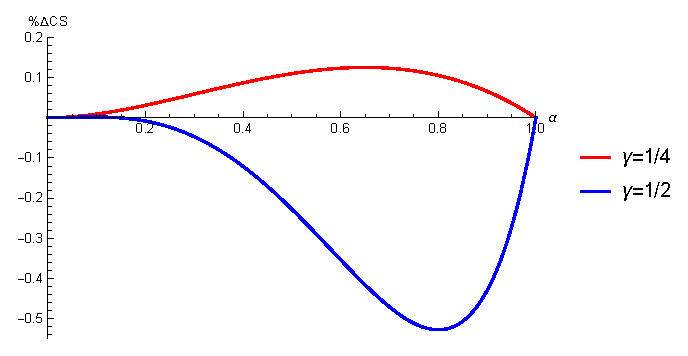
\includegraphics[scale=0.9]{Plots/Bertrand_CS.eps}
\caption{Difference in consumer surplus between \\informative communication (separation) and market signaling}\label{fig:cs2}
\end{figure}


\end{example}

%%%%%%%%%%%%%%%%%%%%%%%%%%%%%%%%%%%%%%%%%%%%%%%%%%%%%%%%%%%%%%%

\section{Conclusion}
By considering imperfect information about the willingness to collude of managers, we introduce a direct motive for communication among managers and show that this communication can be credible in the presence of antitrust fines on both managers and owners.  The analysis highlights the importance of a balance between antitrust fines faces by managers and by owners as well as the non-monotonic effect that antitrust fines have on the likelihood of communication equilibria. 

Whether there is direct communication or indirect communication via market actions, signals are costly. With direct communication, antitrust fines shapes incentives to communicate; with indirect communication, signaling one's willingness to collude via high prices may lead to a loss when the other manager is myopic or unwilling to collude. Preventing communication may induce managers to signal via market actions their willingness to collude, but not always to the benefit of consumers. Indeed, while patient managers will tend to set prices lower than the negotiated prices under communication, the myopic managers will set a higher price than when there is communication: the average price may be higher with tacit collusion. 
 


%%%%%%%%%%%%%%%%%%%%%%%%%%%%%%%%%%%%%%%%%%%%%%%%%%%%%%%%%%%%%%%
\bibliographystyle{agsm}
\bibliography{collusion.bib}
%%%%%%%%%%%%%%%%%%%%%%%%%%%%%%%%%%%%%%%%%%%%%%%%%%%%%%%%%%%%%%%
\appendix
\section{Nash Bargaining}\label{app:HS}
%
In \cite{Harsanyi1972}, the set of players coincides with the set of type-players (hence if there are two individuals, each with two types, there are four `players'). In our model, the set of players is $N:=\{ij:i\in\{0,\delta\},j\in\{1,2\}\}$, and each type-player $ij$ has probability $q_{ij}$.  For instance, if only types $\delta$ decide to communicate, the prior beliefs at the time of communication are $q_{0j}=0,q_{\delta j}=1$ for $j\in\{1,2\}$, while if all types communicate, $q_{0j}=1-\alpha,q_{\delta j}=\alpha$ for $j\in\{1,2\}$. 

We list elements of sets or vectors by first the types of manager $1$ and then types of managers $2$, for instance, $N=\{01,\delta 1, 02,\delta 2\}$, $q=(q_{01},q_{\delta 1},q_{02},q_{\delta 2})$.

Let $\Sigma(q)$ be the set of Grimm-trigger strategies that are perfect Bayesian equilibria given the belief structure $q$ and let $U_{ij}(\sigma)$ be the per-period payoff of player $ij$ if strategy $\sigma$ is played. The set $\Sigma(q)$ is the relevant set of decisions in the bargaining, while in the absence of agreement, the default outcome is to play each period the static game equilibrium $p^c$.

For instance, if only patient managers communicate, the set $\Sigma$ consists of a collusive price $p^*$ together with the threat to revert to $p^c$ if anything but $p^*$ is played in previous periods. If all types communicate, the set $\Sigma$ consists of first period prices $p^*_0(1);p^*_\delta(1)$, one for each type, together with the following continuation strategies. For type $\delta$, play at time $2$, $p^{**}$ if the vector of prices is $(p^*_\delta(1),p^*_\delta(1))$, but play the Grimm-trigger strategy $p^{c}$ if the vector of prices is not $(p^*_\delta(1),p^*_\delta(1))$. For type $0$, play $p^*_0(1)$ that is a best response to $\p^*(1)$ given the belief structure $(1-\alpha,\alpha,1-\alpha,\alpha)$, and play $p^c$ for each period from  time $2$. The condition $p^*_0(1)=BR(\p^*)$ is required for incentive compatibility in the first period.

\cite{Harsanyi1972} show that there exists a unique solution satisfying a series of axioms\footnote{%
The original Nash axioms of Player Symmetry, Efficiency, Irrelevant Alternatives, together with new axioms of Type Symmetry, Splitting Types and Mixing Basic Probability Matrices.
} and that this solution is also the Bayesian-Nash equilibrium outcome of a non-cooperative bargaining game. In our model the Harsanyi-Selten solution solves
\[
\max_{\sigma\in\Sigma(q)}\prod_{ij\in N} (U_{ij}(\sigma)-(\pi^c)^2)^{q_{ij}}.
\]
In the case of a separating equilibrium, this solution coincides with the solution in the text. Indeed, $q=(0,1,0,1)$ in the case of separation. This is not the case when there is pooling as the belief structure is $(1-\alpha,\alpha,1-\alpha,\alpha)$ while we use the structure $(0,1,0,1)$, which is more consistent with other generalizations of the Nash bargaining solution, as in \cite{Myerson1984,Weidner1992}.



\section{Cost of Effort} % (fold)
\label{sec:cost_of_effort}

In this section, we show that for a cost function for effort function $c(e)=e^{E}/E$, the optimal bonus set by owners in the absence of incentive constraints can be made as small as we want by increasing $E$. It should be clear that our qualitative results are preserved, and we illustrate this in the context of Example \ref{ex1}. Somewhat interestingly, larger values of $E$ increase the set of environments consistent with a separating equilibrium.

\paragraph{Separating Equilibrium.} The managers' optimal actions in competition, collusion and deviation are independent of $E$ and the same as before. However, the optimal effort levels are now $e_i^{c}=(b_i \cdot \pi^{c})^\frac{1}{E-1}$, $e_i^{M}=(b_i \cdot \pi^{M})^\frac{1}{E-1}$, and $e_i^{d}=(b_i \cdot \pi(BR(p^M),p^M))^\frac{1}{E-1}$, for competition, collusion, and deviation, respectively. A manager's utilities are $U^{K}=\frac{E-1}{E}(b_i \cdot \pi^{K})^\frac{E}{E-1}$, where $K\in\{c,M,d\}$. Note that, without these constraints the optimal level of bonuses which maximizes the owners' profits is $b=1/E$.

The upper and the lower bounds of bonuses which allows the separation equilibrium are 
\begin{equation*}
   \left(\frac{E}{E-1}\frac{(1-\delta)f}{(\pi^M)^\frac{E}{E-1}-(\pi^c)^\frac{E}{E-1}}\right)^{\frac{E-1}{E}} \leq  b \leq  \left(\frac{E}{E-1} \frac{f}{(\pi^d)^\frac{E}{E-1}-(\pi^c)^\frac{E}{E-1}}\right)^{\frac{E-1}{E}}
\end{equation*}
When $E=2$, we get the same bounds as in Corollary \ref{cor:sep_bonuses}. Figure \ref{fig:Nbonuses} depicts the optimal level of bonuses which can lead to separation equilibrium when $E=20$.

\begin{figure}[ht]
\centering
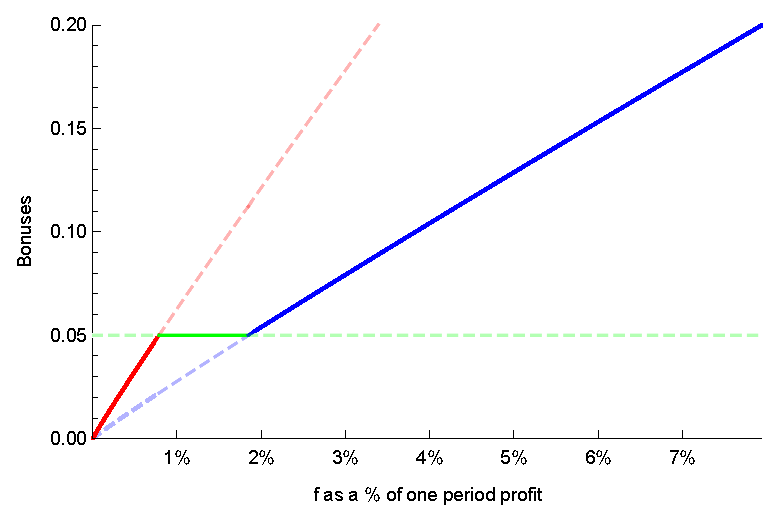
\includegraphics[scale=0.8]{Plots/Bertrand_N_bonuses_diff.eps}
\caption{Bonus levels consistent with a separating equilibrium in the Bertrand example.}\label{fig:Nbonuses}
\end{figure}

We can follow the similar steps for owners and find the separation equilibrium area in fines space. When $E=20$, this area is shown in Figure \ref{fig:Nfines}.

\begin{figure}[ht]
\centering
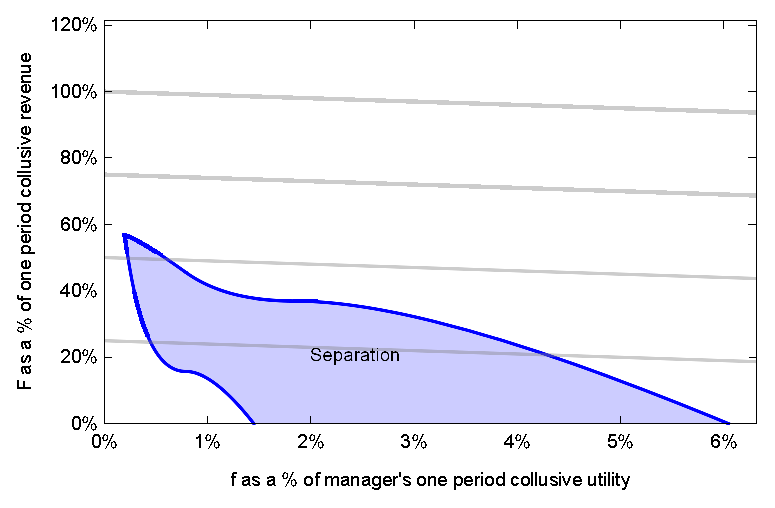
\includegraphics[scale=0.8]{Plots/Bertrand_N_sep_f_F.eps}
\caption{Owner-optimal induced communication strategy of the manager given $f,F$.}\label{fig:Nfines}
\end{figure}

\paragraph{Pooling equilibrium.} The optimal actions of the managers are the same as in the $E=2$ case. In the first period, the optimal level of the efforts are $e^0=b^\frac{1}{E-1}(\alpha \pi(p^d,p^*)-(1-\alpha) \pi(p^d,p^d))^\frac{1}{E-1}$ for the type $0$ and $e^\delta=b^\frac{1}{E-1}(\alpha \pi(p^*,p^*)-(1-\alpha) \pi(p^*,p^d))^\frac{1}{E-1}$ for the type $\delta$ manager. The optimal level of bonuses which leads to pooling equilibrium is given in Figure \ref{fig:Nbonuses_pooling} and the area of pooling equilibrium in the fines space is given in Figure \ref{fig:Nfines_pool_sep}.

\begin{figure}[ht]
\centering
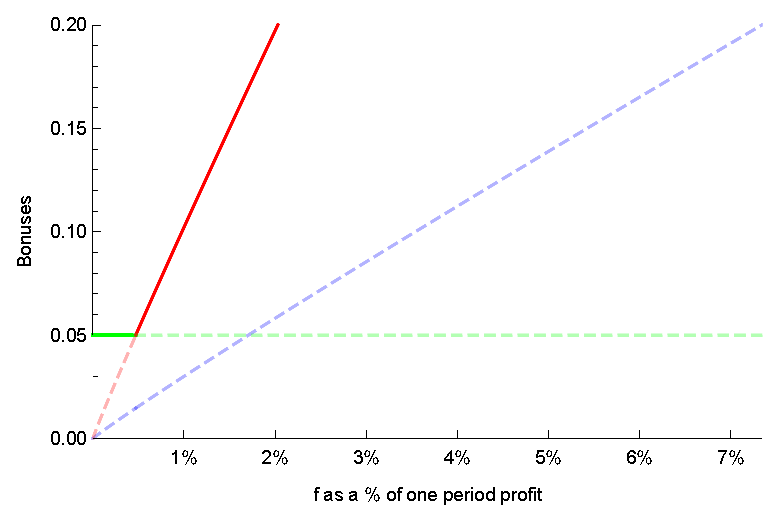
\includegraphics[scale=0.8]{Plots/Bertrand_N_bonuses_diff_bonus_pool2.eps}
\caption{Bonus levels in pooling equilibrium for Bertrand example.}\label{fig:Nbonuses_pooling}
\end{figure}

\begin{figure}[ht]
\centering
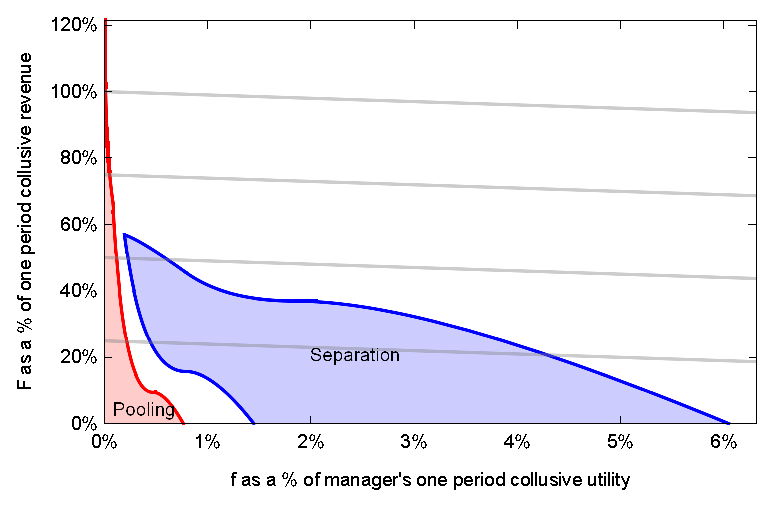
\includegraphics[scale=0.8]{Plots/Bertrand_N_com_f_F_SepvsPool.eps}
\caption{Separating vs pooling equilibrium.}\label{fig:Nfines_pool_sep}
\end{figure}
% section appendix (end)

\clearpage

\section{Penalties on Executives and Undertakings}\label{app:fines}
Data obtained from the following sources (URLs last accessed on 19 May 2020):
\begin{itemize}\setlength\itemsep{-0.5em}
    \item ``Cartels Laws and Regulations 2020,'' Global Legal Insights, \url{https://www.globallegalinsights.com/practice-areas/cartels-laws-and-regulations/}.
    \item ``Cartels 2019,'' Chambers and Partners, \url{https://practiceguides.chambers.com/practice-guides/cartels-2019}.
    \item ``OECD Peer Reviews of Competition Law and Policy, Greece,'' 2018,  \url{http://www.oecd.org/daf/competition/GREECE-OECD-Reviews-of-Competition-Law-and-Policy-2018.pdf}.
     \item ``Annual Report on Competition Policy Developments in Slovenia, 2018,'' OECD, \url{https://one.oecd.org/document/DAF/COMP/AR(2019)30/en/pdf}.
    
\end{itemize}

\begin{table}[htp]
\caption{}
\label{table:fines}
\begin{threeparttable}
\begin{tabular}{llrl}
\toprule
Country & Crime\tnote{a} & Individual Fine\tnote{b}&Corporate Fines\tnote{c} \\
	\midrule	
	\multicolumn{4}{l}{\bf{Individuals and Undertakings - Crime}}\\[0.4em]
	Australia  &Y (10)& A\$500,000 &  $ $ A\$10 million\tnote{e}\\
	Brazil  &Y (2-5)& 1\% - 20 \% of the corporate fine &0.1\%-20\% turnover in Brazil\\
	Canada  &Y (14)& C\$25 million &$ $ C\$25 \\
	Denmark &Y (1.5-6)&$\geq$ DKK$200,000$ & $\geq$ DKK$20$ million, $  10\%$ total turnover \\
	France & Y (4)&€75.000 & $ $ 10\% global turnover  \\
	Germany  & BR (5)& $ $ €1 million & $ $ €1 million or 10\% total turnover \\
	Greece  &Y (5)& €200,000 - 2 million &  $  10\%$ total turnover \\
	Israel  &Y (5)& ISL1 million & $ $ 8\% turnover or ISL100 million \\
	Japan  &Y (5) &¥5 million & $ $¥500 million \\
	Korea  & Y (3) &KRW200 million &  $  10\%$ total turnover  \\
	Norway  & Y (3-6)&  only criminal & $  10\%$ total turnover  \\
	Slovenia  &Y (0.5-5)& €5,000 - €30,000 & $10 \%$ annual turnover\\
	United Kingdom & Y (5)  & unlimited \& Ban (15)& unlimited \\
	United States  &Y (10)& US\$1 million & US\$ 100 million \\
\toprule
	\multicolumn{4}{l}{\bf{Individuals and Undertakings - No Crime}}\\[0.4em]

	China  &N & up to CYN100,000\tnote{d} &  $  10\%$ total turnover\\
	Netherlands &N & $ $ €900,000 &$ $ €900,000 or 10\% global turnover  \\
	Poland  & N& €500,000   & $  10\%$ total turnover \\
	Spain   & N& € 60.000 & $ $ 10 \% total turnover \\
	Sweden  &N& Ban (3-10) & $ $ 10 \%  turnover \\
	Switzerland &N  & CHF100,000 & $ $ 10 \% consolidated 3 yrs turnover\tnote{f} \\
	Turkey   & N & $  5\%$ of corporate &$ $ 10 \% turnover in Turkey  \\
\toprule	
	\multicolumn{4}{l}{\bf{Only undertakings}}\\[0.4em]
	Croatia   &BR (10) &- & $ $ 10 \% total turnover \\
	European Union  &N & - & $ $ 10 \% total turnover \\
	Finland   &N& - &  $ $ 10 \% total turnover\\
	Portugal   &N& - &$ $ 10 \% total turnover  \\
\bottomrule
	\end{tabular}
	\begin{tablenotes}
		\item[a] BR denotes that the executive can face imprisonment only in the case of a Bid Rigging conspiracy. The number in parenthesis is the maximum number of years of imprisonment.
		\item[b] ``Ban'' indicates that the executive can be banned from belonging to a board (interval or maximum number of years in parenthesis). Unless specified, we indicate the maximum duration of the ban.
		\item[c] The maximum fine is indicated.
		\item[d] The fine is for ``obstructing antitrust investigations''.
		\item[e] Maximum three times total benefits, or 10\% group annual turnover if benefits cannot be determined.  
		\item[f] up to 10 percent of the consolidated net turnover realised in Switzerland during the past three financial years (cumulative). 
	\end{tablenotes}
	\end{threeparttable}
\end{table}
\end{document}